\chapter{Must-Alias Analysis: Logical Model}\label{chapter:must-logic}
%A Datalog Model of Must-Alias Analysis

\epigraph{Logic, my dear Zoe, merely enables one to be wrong with authority.}{\textit{The 2nd Doctor} - Doctor Who}


\emph{Pointer analysis} is the backbone of many realistic static analyses, as
it offers a scalable way to model heap behavior.  Pointer analysis typically
comes in two flavors: \emph{alias analysis}, which computes program expressions
that may alias, i.e., refer to the same heap object, and \emph{points-to
analysis}, which computes the heap objects that program variables and
expressions may refer to.

A \emph{must-alias} (or \emph{definite-alias}) analysis computes alias
relationships (between program expressions) that are guaranteed to always hold
during program execution. The analysis is typically flow-sensitive, i.e., it
computes information per-program-point, respecting the control-flow of the
program. A must-alias analysis has several applications:

\begin{itemize}
    \item it is useful for %automatic
        optimizations---e.g., constant folding,
		common subexpression elimination, and register allocation;
	\item it can increase the precision of bug detectors: Nikoli\'{c} and
		Spoto~\cite{ictac:2012:Nikolic} report that a must-alias
		analysis significantly increases the precision of both a null-reference
		detector (46\% fewer warnings) and a non-termination detector (11\%
		fewer warnings). Earlier work has reported similar
		benefits~\cite{isola:2008:Ma};
	%\item it can be used as an internal component in other analyses. For
		%instance, the \textsc{Doop} framework for analysis of Java
		%bytecode~\cite{oopsla:2009:Bravenboer} uses a must-alias analysis in
		%order to perform ``strong updates'' at instructions that modify the
		%heap. Earlier work has used must-alias analysis to similar
	%  benefit~\cite{pldi:1994:Emami,popl:1998:Jagannathan}.
	\item it can be used as an internal component as part of a more complex
		analysis. For instance, must-alias results may enable an analysis to
		perform ``strong updates'' at instructions that modify the heap.
		Earlier work has used must-alias analysis to similar
		benefit~\cite{pldi:1994:Emami,popl:1998:Jagannathan}.
	%% \item it can be invaluable for better program understanding; the results of
	%%	a must-inference are guaranteed facts, of immediate value to the human
	%%	programmer.
	%% \item it is ideal for bug detection that traditionally has a high
	%% 	false-warnings rate. For instance, a may-analysis for null pointer
	%% 	dereferences (either in may-alias or may-point-to form) is rarely of
	%% 	engineering value, due to the preponderance of false warnings. In
	%% 	contrast, a must-analysis for the same problem yields very few
	%% 	warnings, but virtually all of them are actionable.
\end{itemize}

To illustrate must-alias reasoning, consider 
%% The output of a must-alias analysis consists of must-alias pairs: expressions
%% that are guaranteed to point to the same object.
%Figure~\ref{fig:example}.
the code below. In this example, \code{a2.next} and \code{a1} form an alias pair
after line 8. (Other alias pairs include \code{a1.next} and \code{null} after line 7,
\code{a2.next.next} and \code{a2} after line 11, and more.)
Alias pairs are established via direct
variable assignments, calls, as well as heap stores and loads. A must-alias analysis
has to report aliases only when they are guaranteed to hold, and needs to
invalidate them on store instructions or method calls that may change the
fields of objects pointed by subexpressions in an alias pair.

%\code{a1.next} is an alias for \code{a3} on (i.e., after) line 14.  However, line
%15 invalidates that alias pair and instead establishes an aliasing relationship
%between \code{a1.next} and \code{a2}.

%%%% MANUAL PLACEMENT
%\begin{figure}[htb!p]
\vspace{-0.5cm}
\begin{minipage}[l]{3in}
\begin{javacode}
class Node {
	Node next;
	Node(Node next) { this.next = next;	}
	void wrap() { next.next = this;	}
}
void main() {
	Node a1 = new Node(null);
	Node a2 = new Node(a1);
	Node a3 = new Node(null);
	a1.next = a3;
	a2.wrap();
}
\end{javacode}
\end{minipage}
%\caption{Simple illustration of must-alias inferences. }
%\label{fig:example}
%\end{figure}

For instance,
line 10 invalidates the alias pair \code{a1.next} and \code{null}. However, the analysis
is sound (i.e., it remains a must-analysis) if it also invalidates
alias pairs for expressions involving \code{a2.next} or \code{a3.next}. The base
specification of a must-alias analysis has to integrate such soundness safeguards,
while interplay with other analyses (e.g., a may-not-alias analysis) can lead
to more inferences.


%% A must-analysis for
%% pointers is invaluable for automatic optimizations, , as
%% well as for better program understanding: the results of a
%% must-inference are guaranteed facts, of immediate value to the human
%% programmer.  Furthermore, must-analyses are ideal for bug detection
%% that traditionally has a high false-warnings rate. For instance, a
%% may-analysis for null pointer dereferences (either in may-alias or
%% may-point-to form) is rarely of engineering value, due to the
%% preponderance of false warnings. In contrast, a must-analysis for the
%% same problem yields very few warnings, but virtually all of them are
%% actionable.

%% The vast majority of pointer analysis techniques that have appeared in
%% the recent research literature (e.g.,
%% \cite{mattmight:Yong:1999:Pointer,pldi/BerndlLQHU03,cc/KastrinisS13,antgrasshopper,article:2005:Milanova,pldi/WhaleyL04,pldi/SridharanB06})
%% are \emph{may-analyses}. That is, the techniques attempt to
%% \emph{over-approximate} the (unattainable) fully precise result.  All
%% possible alias pairs are guaranteed to be included in the outcome of a
%% may-alias analysis. All possible abstract objects that may be
%% referenced by a variable are included in the variable's may-point-to
%% set. However, spurious inferences 
%% %(which will never occur in program execution) 
%% may also be included in the analysis output.

%% In contrast, an \emph{under-approximate}, \emph{must-analysis} is
%% often desirable. A must-analysis computes aliasing or points-to
%% relationships that are guaranteed to always hold during program
%% execution, at the cost of missing some inferences.


%% In practice, a must-analysis for pointers is often a must-alias
%% analysis, and not a must-point-to analysis. 
%% %Aliasing relationships are more generally provable from local
%% %inspection of the program text, whereas
%% Points-to facts are harder to establish than aliasing relationships in
%% a conservative must- fashion. The difficulty is dual: First, the
%% creation sites of objects are often far from their use sites, making
%% the establishment of must-point-to relationships unlikely. Second,
%% must-point-to reasoning requires careful modeling of abstract
%% vs. concrete objects. For instance, for techniques such as
%% \emph{strong updates} (i.e., replacing the value of an object field at
%% a store instruction) it is not sufficient to know the abstract
%% object that the base expression must-point-to, since the abstract
%% object may conflate many concrete objects during program execution,
%% and only one of them will have its field updated.

%% In this work, we present a data structure that dramatically speeds up
%% the performance of must-alias analysis.  The insights behind the data
%% structure are quite general. We exploit two properties to get high
%% efficiency. First, must-alias sets are \emph{equivalence classes}
%% (must-alias is a symmetric, transitively-closed relation, unlike
%% typical may-alias).  Second, complex program expressions (i.e.,
%% \emph{access paths} of the form ``\args{var}(\args{.fld})*'') do not
%% need to be represented explicitly, but can instead be implicit, and
%% expanded when needed and up to the extent that must-alias information
%% exists for them.

In this work, we present a simple declarative model of a must-alias
analysis over access paths (i.e., expressions of the form
``\args{var}(\args{.fld})*'').  The model underlies the implementation
of must-alias analysis in the \textsc{Doop}
framework~\cite{oopsla:2009:Bravenboer}, which expresses several
analyses of Java bytecode using Datalog specifications. \textsc{Doop}
employs must-alias analysis as an enhancer of its standard array of
may-analyses---e.g., in order to enable ``strong updates''.

The model is interesting in a few different ways:

\vspace{-1mm}
\begin{itemize}
\item It is an instance of a flow-sensitive analysis in Datalog. As such,
  it introduces idioms and patterns also used in a multitude of other
  (current or future) analyses in \textsc{Doop}.
  
\item The analysis is minimal, yet models the core features of a
  general must-alias analysis in a handful of declarative rules.  In
  this way, the analysis semantics are easily understood and can be
  further enhanced. The rules allow configurability and employ several
  techniques for conciseness and power. The use of context, in particular,
  is crucial: the analysis introduces context variables, much like in
  traditional may analyses (e.g., \cite{pldi:2013:Kastrinis,article:2015:Smaragdakis}), yet
  uses the context highly unconventionally. Context is used as ``fuel'',
  to guarantee the ``must'' nature of the analysis: must-alias inferences
  are propagated inter-procedurally, with context extended for every
  call. When maximum context depth is reached, inferences cannot propagate
  any further.

\item The analysis gives rise to several observations, concerning the
  representation of equivalence relations in a Datalog engine,
  and the need for implicit encodings of aliasing.
\end{itemize}

%% The first element of the work is an analysis model that integrates
%% the essential features of a general must-alias analysis (e.g., context
%% sensitivity). This model condenses a full-fledged implementation
%% into a core of a handful of declarative rules, written in the Datalog
%% language. In this way, the analysis semantics and characteristics are
%% easily understood and can be further enhanced. Indeed, the analysis
%% core we present is the basis of a much larger (over 300 Datalog rules)
%% must-alias analysis implementation already in active use in the
%% \textsc{Doop} static analysis framework~\cite{oopsla:2009:Bravenboer}
%% for Java bytecode.

%% Based on this declarative analysis model, it is possible to identify
%% the main concepts and operations of our must-alias analysis. Namely,
%% each instruction maintains a set of \emph{alias classes}: equivalence
%% classes of access paths that are certain to be aliased at the given
%% program point. The operations performed over the sets of alias classes
%% are a) removing an access path from a set and inserting it into
%% another; b) producing a set of alias classes by intersecting two
%% existing sets of alias classes. These operations, together with
%% standard properties of the must-alias analysis (e.g., that aliased
%% access paths remain aliased if extended with the same suffix, or that
%% alias sets are equivalence classes) give rise to the second element of
%% our work: a graph-based data structure for a highly-efficient
%% representation of sets of alias classes. We base a re-implementation
%% of the must-alias analysis on the specialized data structure and show
%% that it achieves dramatic speedup (typically over 20x) compared to the
%% original.
%% %REVIEW

%% \textsc{MaDoop}: a general must-alias
%% analysis framework, with significant configurability. Our framework is
%% implemented in the Datalog language, as an extension of the
%% . The
%% \textsc{MaDoop} framework comprises some-300 logical rules, as well as
%% scaffolding code for the low-level (flow-sensitive) modeling of Java
%% bytecode as logical relations.  However, the essence of the framework,
%% for a minimal input language, is well-captured in a small number of
%% rules, which we present in detail in this paper. 

%% %% The framework specification is quite modular: extra functionality can be
%% %% supported as additional rules. Furthermore, the framework can be configured to
%% %% achieve different trade-offs of inference power (i.e., more alias pairs
%% %% established) and scalability. For instance, the framework allows control over
%% %% context creation, access path creation, and more.

%% %An important
%% %dimension, which our work explores, is that of context-sensitivity.
%% %Context-sensitivity is a concept of diminished value for an alias
%% %analysis, since alias pairs already offer a summary of a function's
%% %behavior, and this summary is customized at call sites. However, we
%% %discuss interesting ways in which context-sensitivity can be
%% %profitable in the must-alias analysis setting. 
%% Finally, as is common in practice, a must-alias analysis employs a
%% may-analysis as a pre-processing step. Our framework concisely
%% captures all the points at which may- information interfaces with
%% must- information. Furthermore, we analyze and quantify the impact of
%% the choice of may-analysis on the effectiveness of the must-alias
%% analysis.


%% A major benefit of a must-alias analysis is its
%% \emph{incrementality}. In a well-specified must-alias analysis,
%% soundness is not compromised if only a portion of the
%% program-under-analysis or its libraries are available.  This key
%% element is emphasized in our declarative model.  We control
%% the program points where the full analysis applies and leverage
%% context-sensitivity to allow analysis of other program points.

%% %%SPACE
%% %In essence, our analysis infers normal must-alias relationships for a
%% %user-selected core part of the program, and infers conditional,
%% %context-qualified must-alias relationships for other parts that
%% %interact with the core program.


%% Our data structure is effectively a symbolic abstraction of the
%% program's heap---as a directed graph.  We invent for each variable a
%% graph node: an abstract object that represents ``the object that the
%% variable points to''. This abstract object represents at most one
%% concrete object, unlike traditional abstractions that map multiple
%% concrete objects to one abstract. Whenever a must-alias inference is
%% made, the corresponding abstract objects are merged: the two abstract
%% objects have to correspond to the same concrete one. Access paths are
%% represented implicitly, as regular paths that follow object fields
%% through our symbolic heap. All operations over the graph arising
%% during a must-alias analysis (esp. the intersection of graphs) are
%% performed highly efficiently.
%% 
%% We implement the data structure in two settings: imperatively, in
%% Java, with destructive updates (upon aliasing, abstract objects are
%% collapsed together) and purely functionally (upon aliasing, abstract
%% objects are related in an associative structure). The latter is
%% suitable for a declarative implementation, in the Datalog language.
%% We show that the data structure yields large performance improvements
%% compared to an explicit representation of alias pairs. The imperative
%% version achieves a speedup of up to two orders of magnitude, with the
%% declarative implementation nearly matching it in most cases.  As a
%% result, the running time of a realistic must-alias analysis becomes
%% small---a few tens of seconds for large benchmarks and the full Java
%% library.

%% Overall, our work:

%% \begin{itemize}
%% %\item offers the first static handling of Java reflection that 
%% % exhibits both high empirical soundness and performance for
%% % sophisticated analyses and large-scale benchmarks, with no
%% % extra inputs;
%% \item models a general must-alias analysis framework over access paths and the
%% 	primitive operations (e.g., set intersection) that a must-alias analysis
%% 	needs to perform;
%% %\item applies the framework, with extensions for fully realistic treatment of
%% %	language features, to Java bytecode;
%% \item presents an efficient data structure for representing must-alias analysis
%% 	inferences and efficiently encodes operations over that structure;
%% \item quantifies the benefits of the new data structure in different
%% 	implementation settings.
%% \end{itemize}

%%SPACE
%In the rest of the paper, we present an example for illustration of
%must-alias reasoning (Section~\ref{sec:example}), show our analysis
%algorithm (Section~\ref{sec:model}), discuss its parametric character
%and configurability options (Section~\ref{sec:configurability}),
%analyze tradeoffs experimentally (Section~\ref{sec:experiments}),
%detail related work (Section~\ref{sec:related}) and conclude
%(Section~\ref{sec:conclusions}).


%% \section{Background and Example}
%% \label{sec:example}
%% 
%% %% We illustrate some basic concepts of must-alias reasoning with a small example,
%% %% also used in later sections to illustrate our data structures and algorithms.
%% 
%% %%%% MANUAL PLACEMENT
%% \begin{figure}[htb!p]
%% \vspace{-0.4cm}
%% \begin{minipage}[l]{3in}
%% \begin{javacode}
%% class A { 
%%   A next; 
%%   B member;
%% 
%%   A(A next, B member) {
%%     this.next = next;
%%     this.member = member;
%%   }
%% 
%%   void foo(A a) {
%%     member.container = a;
%%   }
%% }
%% 
%% class B {
%%   A container;
%%   B(A container) { 
%%     this.container = container; 
%%   }
%% }
%% 
%% public class Test {
%%   public static void main(String[] args) {
%%     B b1 = new B(null);
%%     A a1 = new A(null, b1);
%%     A a2;
%%     if (args != null) 
%%       a2 = new A(null, b1);
%%     else
%%       a2 = new A(a1, b1);
%%     b1.container = a2;
%%     a1.foo(a1);
%%   }
%% }
%% \end{javacode}
%% \end{minipage}
%% \caption{Simple illustration of must-alias inferences. }
%% \label{fig:example}
%% \end{figure}
%% 
%% Consider the small Java program in Figure~\ref{fig:example}. Even at this size,
%% inspecting the program requires human effort. A must-alias analysis can provide
%% useful information to tools and humans alike. The output consists of must-alias
%% pairs: expressions that are guaranteed to point to the same object. (More
%% precise definitions follow in Section~\ref{sec:model}.) For instance,
%% \code{a1.member} and \code{b1} form an alias pair for almost the entire body of
%% method \code{main}.  Alias pairs are established by direct variable assignments
%% (which are plentiful in a compiler intermediate language, although less so in
%% original source code), as well as heap stores and loads. A must-alias analysis
%% has to report aliases only when they are guaranteed to hold, and needs to
%% invalidate them on store instructions or method calls that may change the
%% fields of objects pointed by subexpressions in an alias pair. In
%% Figure~\ref{fig:example}, \code{b1.container} is an alias for \code{a2} on (i.e.,
%% after) line 31. However, the analysis needs to recognize that line 32
%% invalidates that alias pair. Line 32 instead establishes an aliasing
%% relationship between \code{b1.container} (as well as \code{a1.member.container})
%% and \code{a1}. The analysis remains sound (i.e., safely under-approximate) if the
%% earlier \code{b1.container} $\sim$ \code{a2} alias pair is invalidated, regardless
%% of whether the new alias pair (\code{b1.container} $\sim$ \code{a1}) is
%% established, via inter-procedural reasoning, on line 32. 
%% 
%% %% Such invalidation can take place either conservatively, at all method call
%% %% points, or by use of a may-analysis, which informs the must-analysis that the
%% %% call to \code{foo} will result in changes to the \code{container} field of an
%% %% object.
%% 
%% Other aliasing relationships hold throughout the program. Establishing them
%% often requires some inter-procedural reasoning---e.g., to see the aliasing
%% effects of the constructor call on lines 25, 28, or 30. Constructors feature
%% prominently in the example, since they are one of the best sources of
%% must-alias information in a typical program.


\section{Must-Alias Analysis Model}
\label{sec:model}

%% The analysis remains sound
%% (i.e., safely under-approximate) if the earlier \code{b1.container} $\sim$
%% \code{a2} alias pair is invalidated, regardless of whether the new alias pair
%% (\code{b1.container} $\sim$ \code{a1}) is established, via inter-procedural
%% reasoning, on line 32. 

%% Such invalidation can take place either conservatively, at all method call
%% points, or by use of a may-analysis, which informs the must-analysis that the
%% call to \code{foo} will result in changes to the \code{container} field of an
%% object.

%% Other aliasing relationships hold throughout the program. Establishing them
%% often requires some inter-procedural reasoning---e.g., to see the aliasing
%% effects of the constructor call on lines 25, 28, or 30. Constructors feature
%% prominently in the example, since they are one of the best sources of
%% must-alias information in a typical program.



%% The model is written in the Datalog language, often used to specify
%% program analyses~\cite{repsdb,aplas/WhaleyACL05,oopsla:2009:Bravenboer}. The
%% purpose of the model is dual. First, it allows us to reason about must-alias
%% analysis without dealing with the details of a specific implementation. At the
%% specification level (which the Datalog model captures well) we can see that a
%% must-alias analysis algorithm needs to perform some standard operations:
%% maintain equivalence relations, intersect must-alias information, etc.

%% Second,
%% the model matches well the implementation of the must-alias analysis in the
%% \textsc{Doop} framework, which we will compare against in our experiments.

%% Since the early work of Reps~\cite{repsdb}, Datalog has been repeatedly used to
%% express program analysis algorithms (e.g.,
%% \cite{aplas/WhaleyACL05,madsen13javascript,pldi/ZhangMGNY14}).  The language
%% ideally captures the usual program analysis notion of monotonic iteration until
%% fixpoint.

%% Datalog rules infer more facts
%% from combinations of previously established facts, with variables
%% implicitly quantified existentially.  A rule of the form
%% ``\rel{Head}{x,y} \rulearrow{} \rel{P}{x,z}, \rel{Q}{y,z}.''  means
%% that if values for \args{x,y,z} can be found so that \rel{P}{x,z} and
%% \rel{Q}{y,z} are simultaneously true, then \rel{Head}{x,y} is
%% inferred. Syntactically, the left arrow symbol (\rulearrow) separates
%% the inferred facts (i.e., the \emph{head} of the rule) from the
%% previously established facts (i.e., the \emph{body} of the rule). For
%% our analysis to be expressed in Datalog, we assume that the
%% program-under-analysis is represented as input relations (typically
%% implemented as database tables) that encode its different
%% elements. Such pre-processing is a relatively straightforward
%% one-to-one translation.

We next present a minimal Datalog model of an inter-procedural must-alias analysis
algorithm on a static-single assignment (SSA) intermediate language.

\subsection{Intermediate Language / Analysis Schema}

%% We show our algorithm on a minimal static-single assignment (SSA) intermediate
%% language.%% \footnote{That is, every local variable is assigned exactly once in
%% the input program. For variables with multiple assignments in the original
%% source code, the merging of their values is indicated by a $\phi$ node.
%% \args{var = $\phi$(var1,var2)} signifies that the value of \args{var} can be
%% either of the two values on the right-hand side. For the purposes of static
%% analyses, like ours, that do not track path conditions, it is not relevant
%% which of the two values is actually picked.}

%%SPACE
%% with a) a ``move'' instruction for copying between local variables; b) a
%% ``phi'' instruction for merging of single-assignment variables; c) ``store''
%% and ``load'' instructions for writing to the heap (i.e., to object fields); and
%% d) a ``virtual method call'' instruction that calls the method of the
%% appropriate signature defined in the dynamic class of the receiver object. To
%% be usable, the intermediate language is expected to also contain other
%% features, such as object allocation, which do not play a role in the core
%% must-alias analysis. Furthermore, 
The language can be enhanced with features such as arrays, static members and
calls, exceptions, etc. to be a full-fledged intermediate language.
Indeed, our actual analysis implementation is on the Jimple intermediate
language of the Soot framework~\cite{cascon:1999:Vall},%cc:2000:Vall},
which
models all features of Java bytecode. Yet the core of the analysis is
represented well in the minimal language.

\begin{figure}[tb!p]
%\begin{center}
\hspace{-2.5mm}
\begin{tabular}{l}
%%   \small $V$ is a set of program variables    \\
%%   \small $M$ is a set of method identifiers \\
%%   \small $S$ is a set of method signatures (name+types)\\
%%   \small $F$ is a set of fields \\
%%   \small $I$ is a set of instructions \\
%%   \small $T$ is a set of types \\
%%   \small $C$ is a set of contexts \\
%%   \small $A$ is $V$$(.F)*$: a set of access paths \\
  %%    \small $\mathbb{N}$ is the set of natural numbers \\
  \begin{small}
\begin{tabular}{r l r l}
	$V$: & program variables &  $M$: & method identifiers \\
	$S$: & method signatures &  $F$: & fields \\
	$I$: & instructions &  $T$: & types \\
	$C$: & contexts &  $\mathbb{N}$: & natural numbers \\
  \multicolumn{4}{c}{$A$: access paths of the form $V$$(.F)*$} \\
\end{tabular}  \end{small} \\
\hhline{=}
\hspace{-3mm}
\begin{tabular}{l l}
%\rel{Alloc}{i: I, var: V, heap: H, inMeth: M}  & \args{\# i: var = new ...} \\
\rel{Move}{i: I, to: V, from: V}                & \args{\# i: to = from} \\
\rel{Load}{i: I, to: V, base: V, fld: F}       & \args{\# i: to = base.fld}\\
\rel{Store}{i: I, base: V, fld: F, from: V} & \args{\# i: base.fld = from} \\
\rel{Call}{i: I, base: V, sig: S}              & \args{\# i: base.sig(..)}   \\
\rel{Phi}{i: I, to: V, from1: V, \ldots}       & \args{\# i: to = $\phi$(from1, \ldots)}\\
\rel{Next}{i: I, j: I}   & \args{\# j is CFG successor of i}\\
\end{tabular}\\
%\cline{1-1}
%\hhline{=}
\\
\hspace{-3mm}
\begin{tabular}{l}
  \rel{FormalArg}{meth: M, n: $\mathbb{N}$, arg: V}\\
  \rel{ActualArg}{invo: I, n: $\mathbb{N}$, arg: V} \\ 
  \rel{FormalRet}{instr: I, meth: M, ret: V} \\
%  \rel{ActualRet}{invo: I, var: V} \\ 
  \rel{ThisVar}{meth: M, this: V} \\
  \rel{LookUp}{type: T, sig: S, meth: M} \\
  \rel{InMethod}{instr: I, meth: M} \\
  \altrel{Resolved}{var: V, type: T} \\
  \altrel{RootMethod}{meth: M} \\
\end{tabular}
\\
\hhline{=}
%\cline{1-1}
\rel{MustAlias}{inst: I, ctx: C, ap1: A, ap2: A} \\
\rel{MustCallGraphEdge}{invo: I, ctx: C, toMth: M, toCtx: C} \\
\rel{Reachable}{ctx: C, meth: M} \\
\hhline{=}
\cons{AP}{access path expression}{ap: A} \\
\cons{PrimeAP}{ap: A}{newAp: A} \\
\cons{UnprimeAP}{ap: A}{newAp: A} \\
\cons{NewContext}{invo: I, ctx: C}{newCtx: C} \\
%% \hhline{=}
%% \begin{tabular}{llll}
%% \altrel{Resolved}{var: V, type: T} &&& \altrel{MayAlias}{var1: V, var2: V} \\
%% \altrel{CallMayStoreToField}{invo: I, fld: F} &&& \altrel{RootMethod}{meth: M} \\
%% \end{tabular}
%\\
%\cline{1-1}
\end{tabular}
%\end{center}
%% \caption[]{Our domain, input relations (\relname{Move}, ...),
%%   computed relations (\relname{MustAlias}, ...), and constructors
%%   (\consname{AP}, ...). 
%% %% and configuration predicates (\altrel{Resolved}, ...).  
%%   The input relations are of two kinds:
%%   relations encoding program instructions
%% %%(the form of the instruction is shown in a comment)
%%   and relations encoding type system and other environment
%%   information.}
\caption[]{Our domain, input relations (\relname{Move}, ...),
  computed relations (\relname{MustAlias}, ...), and constructors
  (\consname{AP}, ...).}
\label{fig:input}
\end{figure}


Figure~\ref{fig:input} shows the domain of the analysis (i.e., the
different value sets that constitute the space of our computation) and
three different groups of relations. 
%% four
%%%SPACE
%(These relations are explained in
%more detail below, but their declarations and type signatures can be
%handy for reference.)  The first group (starting with \relname{Move})
%contains relations representing the input language instructions and
%other program text information, such as types and member lookup.  The
%second group (starting with \relname{MustAlias}) contains relations
%computed by our algorithm. The third group (starting with
%\consname{AP}) contains functions that produce new objects, either
%contexts or access paths. The fourth group (starting with
%\altrelname{Resolved}) also lists input relations, but of a different
%kind. These are expected to either be supplied by the user for
%analysis configuration purposes, or to be computed by an earlier-run
%may-analysis.

\paragraph{Input Relations.}
The input relations correspond to our intermediate language features.  They are
logically grouped into relations that represent instructions and relations that
represent name-and-type information.
%% For instance, the \relname{Move}
%% relation represents instructions that assign a local variable to another. There
%% are similar input relations for other instruction types (\relname{Load},
%% \relname{Store}, and \relname{Call}, for reading/writing heap object fields
%% and for virtual calls, respectively).
In particular, the \relname{Phi} relation captures
$\phi$ instructions, for the SSA form of our intermediate language. The
\relname{Next} relation expresses directed edges in the control-flow graph
(CFG): \rel{Next}{i,j} means that \args{i} is a CFG predecessor of \args{j}.

Similarly, there are relations that encode type system, symbol table, and
program environment information---e.g., \relname{FormalArg}, \relname{ActualArg},
\relname{FormalRet}, \relname{ThisVar}. 
%% %% These are mostly straightforward. 
%% For instance, \relname{FormalArg} shows which variable is a formal argument of
%% a given method at a certain index (i.e., the $n$-th argument).
%% %The relation is a function from the first two arguments to the third.
%% \relname{ActualArg} is
%% similar, but at a method invocation site.  \relname{FormalRet} combines
%% information on the return variable of a function with the index of the return
%% instruction. 
%% %  \relname{ActualRet} is a function of its first argument (a method
%% %  invocation site) and returns the local variable at the call site
%%   %  that receives the method call's return value.
%% \relname{ThisVar} returns the \code{this} variable of a method.
The input intermediate language program is assumed to
be in a single-return form, for each method.
\relname{LookUp}
%is a function from its first two arguments to the third. It
matches a method signature to the actual method definition inside a
type.  \relname{InMethod} is a function from instructions to their
containing methods. \relname{Resolved} is a predicate that can be
computed by an external call-graph or may-point-to analysis: it holds
variables that are determined to only point to objects with a unique
dynamic type, so that virtual method calls are resolved. (Note that
the form of the predicate is context-insensitive, yet the analysis
that computes it may be context-sensitive, for increased
precision---the contexts are merely projected out.)  Finally,
\relname{RootMethod} is a predicate over methods, used to start
must-alias reasoning from a user-selected set of methods.
%% As we will see, our analysis algorithm will venture beyond these root methods
%% only to the extent that its context constructor allows.

\paragraph{Computed Relations.}

Figure~\ref{fig:input} also shows the computed relations of our must-alias
analysis. The first relation, \relname{MustAlias}, is also the main output of
the analysis. The relation is defined on access paths, i.e., expressions of the
form ``\args{var}(\args{.fld})*''.  The meaning of \rel{MustAlias}{i, ctx,
ap1, ap2} is that access path \args{ap1} aliases access path \args{ap2} (i.e.,
they are guaranteed to point to the same heap object, or to both be \code{null})
right after program instruction \args{i}, executed under context \args{ctx},
provided that the instruction is indeed executed under \args{ctx} at program
run-time. The two access paths are said to form an \emph{alias pair}.  
 
%% The introduction of access paths and contexts raises
%% natural questions: how complex can access paths get?  What is a
%% context and what does it mean for it to occur at run-time?  We
%% postpone the full treatment of these questions until
%% % our discussion of analysis configurability in
%% Section~\ref{sec:configurability}.

Other computed relations represent intermediate results of the analysis.
\relname{MustCallGraphEdge} holds information for fully-resolved virtual
calls: invocation site \args{invo} will call method \args{toMth} under the
given contexts.  \relname{Reachable} computes which methods and under what
context are of interest to the must-alias analysis.

\paragraph{Constructors.}
We assume a constructor function \consname{AP} that produces access paths. For
instance, inside a logic program, ``\cons{AP}{var.fld1.fld2}{ap}'' means that
the access path \args{ap} has length 3 and its elements are given by the values
of bound logical variables \args{var}, \args{fld1} and \args{fld2}.
We also manipulate access paths with two functions \consname{PrimeAP}
and \consname{UnprimeAP}. \consname{PrimeAP} takes an access path and
returns a new one by ``priming'' the base variable of the
original. \consname{UnprimeAP} reverses this mapping. For instance,
\cons{PrimeAP}{``v.fld''}{``v\textbf{'}.fld''}. \consname{UnprimeAP}
only applies to access paths with primed variables as their
base---otherwise the rule fails to match. Priming and unpriming of
access paths is done at method call and return sites, to mark access
paths that arrive from callers. This is necessary for avoiding
confusion of variables in recursive calls.

Similarly, we construct new contexts using function \consname{NewContext}.  The
definition of this constructor serves to configure the analysis for different
context settings, as discussed later.  If \consname{NewContext} does not return
a value (e.g., because the maximum context depth has been reached), the current
rule employing the constructor will not produce facts.  The constant
\consname{All} is used to signify the initial context.

We shall also use \consname{AP} as a pattern matcher over access paths. For
instance, the expression ``\cons{AP}{\_.fld}{ap}'' binds the value of logical
variable \args{fld} to the last field of access path \args{ap}. (\_ is an
anonymous variable that can match any value.)
%%SPACE
% in a Datalog program.)

Constructors of access paths and contexts are much like other relations. In
practical analyses, the space of access paths and contexts is made finite,
by bounding their length. %, and similarly for contexts.

%%SPACE
%% Therefore, all possible access paths and contexts could be computed prior to
%% the analysis start and supplied as inputs. However, this is unlikely to be
%% desirable in practice, for efficiency reasons, and is limiting in principle: by
%% separating constructors, our model also allows analyses with unbounded access
%% paths and contexts.

%% \paragraph{Configuration Predicates.}
%% The last four elements of Figure~\ref{fig:input} show input predicates that can
%% be used to configure the must-alias analysis.  Predicates \relname{Resolved},
%% \relname{MayAlias}, and \relname{CallMayStoreToField} are expected to be
%% computed by a \emph{may-point-to} analysis, running as a preprocessing step.
%% \relname{Resolved} holds variables that are determined to only point to
%% objects with a unique dynamic type. \relname{MayAlias} reflects whether two
%% variables (in the same method) may point to the same object.
%% \relname{CallMayStoreToField} does a transitive search of all methods that may
%% be called at an invocation site, \args{invo}, looking for store instructions to
%% field \args{fld}.
%%SPACE
%% The power of the must-alias analysis will hinge on the precision of
%% these relations.


\subsection{Analysis Model}

Figure~\ref{fig:rules-must-1} 
%and \ref{fig:rules-must-2} 
shows our analysis model, in four groups of rules. For conciseness, we have
employed some syntactic sugar:
%, which straightforwardly maps to more complex Datalog rules:

\begin{itemize}
\item In addition to conjunction (signified by the usual ``,'' in a rule body)
	our rules also employ disjunction (``;'') and negation (``!''). Negation is
	stratified: it is only applied to predicates that are either input
	predicates or whose computation can complete before the current rule's
	evaluation. We also permit multiple predicates in a rule head, as syntactic
	sugar for replicating the rule body.%% an equal number of times.

\item We use the shorthand \relname{P*} for the reflexive, symmetric,
	transitive closure of relation \relname{P}, which is assumed to be binary.
	For larger arities, underscore (\_) variables are used to distinguish
	variables of a relation that are affected by the closure rule.
	Specifically, \rel{MustAlias*}{i, ctx, \_, \_} denotes the reflexive,
	symmetric, transitive closure of relation \relname{MustAlias} with respect
	to its last two variables.

\item We introduce $\forall$: syntactic sugar that hides a Datalog pattern for
	enumerating all members of a set and ensuring that a condition holds
	universally.\footnote{Emulating universal quantification in Datalog
	  requires ordered domains. 
% In practice, this is not a restriction:
    An arbitrary ordering relation (e.g., by internal id of facts as assigned by
	the implementation) can be imposed on all our domains.} An expression
	``$\forall$\args{i}: \rel{P}{i} \ruleforall{} \rel{Q}{i,...}''  is
	true if \rel{Q}{i,...} holds for all \args{i} such that \rel{P}{i} holds.
	Such an expression can be used in a rule body, as a condition for the
	rule's firing. Multiple variables can be quantified by a $\forall$. Variables
	not bound by $\forall$ remain implicitly existentially
	quantified, as in conventional Datalog. However, the existential quantifier
	is interpreted as being outside the universal one. For instance,
	``$\forall$\args{i,j}: \rel{P}{i,j,k} \ruleforall{}
	\rel{Q}{i,j,k,l}'' is interpreted as ``there exist \args{k,l} such that
	for all \args{i,j} ...''.
\end{itemize}

%% The rules in Figure~\ref{fig:rules-must-1} 
%% %and \ref{fig:rules-must-2}
%% are split into four groups. 
%% %%SPACE
%% %We discuss them in order, next.


\paragraph{Base Rules.}

\begin{figure}[tb!p]
%\begin{center}
\begin{tabular}{l}
%\cline{1-1}
\rel{Reachable}{ctx,m} \rulearrow{} \altrel{RootMethod}{m}, \args{ctx} = \consname{All}.\\
\rule{-2pt}{3ex}

\rel{MustAlias}{i, ctx, \consapp{AP}{from}, \consapp{AP}{to}} \rulearrow{} \\
\tab \rel{Move}{i, to, from}, \rel{InMethod}{i, m}, \rel{Reachable}{ctx,m}. \\
\rule{-2pt}{3ex}

\rel{MustAlias}{i, ctx, ap, \consname{AP}(\args{to})} \rulearrow{} \\
\tab ($\forall$\args{from}: \rel{Phi}{i, to, \ldots, from, \ldots} \ruleforall{} \\
\tab \tab \tab              \rel{MustAlias}{i, ctx, \consapp{AP}{from}, ap}),\\
\tab \rel{InMethod}{i, m}, \rel{Reachable}{ctx,m}. \\
\rule{-2pt}{3ex}

\rel{MustAlias}{i, ctx, \consapp{AP}{to}, \consname{AP}(\args{base.fld})} \rulearrow{} \\
\tab \rel{Load}{i, to, base, fld}, \\
\tab \rel{InMethod}{i, m}, \rel{Reachable}{ctx,m}. \\
\rule{-2pt}{3ex}

\rel{MustAlias}{i, ctx, \consapp{AP}{from}, \consname{AP}(\args{base.fld})} \rulearrow{} \\
\tab \rel{Store}{i, base, fld, from}, \\
\tab \rel{InMethod}{i, m}, \rel{Reachable}{ctx,m}. \\
\rule{-2pt}{3ex}

\rel{MustAlias}{i, ctx, \_, \_} \rulearrow{} \rel{MustAlias*}{i, ctx, \_, \_}. \\

\hhline{=}
%\rule{-2pt}{3ex}

\rel{MustCallGraphEdge}{i, ctx, toMth, toCtx}, \\
\rel{Reachable}{toCtx, toMth} \rulearrow{} \\
\tab \rel{Call}{i, base, sig}, \\
\tab \rel{InMethod}{i, m}, \rel{Reachable}{ctx,m}, \\ 
\tab \altrel{Resolved}{base, type}, \rel{LookUp}{type, sig, toMth}, \\
\tab \cons{NewContext}{i,ctx}{toCtx}. \\
\rule{-2pt}{3ex}


\rel{MustAlias}{firstInstr, toCtx, ap1, ap2} \rulearrow{} \\
\tab \rel{MustCallGraphEdge}{i, ctx, toMth, toCtx}, \\
\tab \rel{InMethod}{firstInstr, toMth}, 
     ($\forall$\args{k} \ruleforall{} !\rel{Next}{k, firstInstr}), \\
\tab ((\rel{FormalArg}{toMth, n, toVar}, \rel{ActualArg}{i, n, var}); \\
\tab \tab (\rel{ThisVar}{toMth, toVar}, \rel{Call}{i, var, \_})), \\
\tab \cons{PrimeAP}{\consapp{AP}{var}}{ap1}, \cons{AP}{toVar}{ap2}. \\
\rule{-2pt}{3ex}


\rel{MustAlias}{firstInstr, toCtx, ap1, ap2} \rulearrow{} \\
\tab \rel{MustCallGraphEdge}{i, ctx, toMth, toCtx}, \\
\tab \rel{InMethod}{firstInstr, toMth}, 
     ($\forall$\args{k} \ruleforall{} !\rel{Next}{k, firstInstr}), \\
\tab ($\forall$\args{j}: \rel{Next}{j, i} \ruleforall{} \\
\tab \tab \tab           \rel{MustAlias}{j, ctx, callerAp1, callerAp2}),\\
\tab \cons{PrimeAP}{callerAp1}{ap1}, \cons{PrimeAP}{callerAp2}{ap2}.\\
\rule{-2pt}{3ex}

\rel{MustAlias}{i, ctx, ap1, ap2} \rulearrow{} \\
\tab \rel{MustCallGraphEdge}{i, ctx, toMth, toCtx}, \\
\tab \rel{FormalRet}{reti, toMth, \_}, \\
\tab (\rel{MustAlias}{reti, toCtx, calleeAp1, calleeAp2}; \\
\tab \tab \rel{MustAlias}{reti, \consname{All}, calleeAp1, calleeAp2}), \\
\tab \cons{UnprimeAP}{calleeAp1}{ap1}, \\
\tab \cons{UnprimeAP}{calleeAp2}{ap2}.\\
\hhline{=}

%\cline{1-1}
%\rel{Reachable}{ctx, meth}, \rel{Reachable}{toCtx, toMeth} \rulearrow{} \\
%\tab \rel{MustCallGraphEdge}{i, ctx, toMeth, toCtx}, \\
%\tab \rel{InMethod}{i, meth}. \\
%\rule{-2pt}{3ex}

%\rel{MustAlias}{i, ctx, ap1, ap2} \rulearrow{} \\
%\tab \rel{MustAlias}{i, \consname{All}, ap1, ap2}, \rel{InMethod}{i, meth}, \rel{Reachable}{ctx, meth}. \\
%\rule{-2pt}{3ex}

\rel{MustAlias}{i, ctx, ap3, ap4} \rulearrow{} \\
\tab \rel{MustAlias}{i, ctx, ap1, ap2}, \\
\tab \cons{AP}{ap1.fld}{ap3}, \cons{AP}{ap2.fld}{ap4}. \\
\hhline{=}
%\cline{1-1}
\rel{MustAlias}{i, ctx, ap1, ap2} \rulearrow{} \\
\tab !\rel{Store}{i, \_, \_, \_}, !\rel{Call}{i, \_, \_},\\
\tab ($\forall$\args{j}: \rel{Next}{j, i} \ruleforall{} 
        \rel{MustAlias}{j, ctx, ap1, ap2}).\\
\rule{-2pt}{3ex}

%% SPACE!
%\rel{MustAlias}{i, ctx, ap1, ap2} \rulearrow{} \\
%\tab \rel{Call}{i, \_, \_}, 
%     ($\forall$\args{j}: \rel{Next}{j, i} \ruleforall{} 
%      \rel{MustAlias}{j, ctx, ap1, ap2}), \\
%\tab \cons{AP}{var1}{ap1}, \cons{AP}{var2}{ap2}.\\
%\rule{-2pt}{3ex}
%\cline{1-1}
\end{tabular}
%\end{center}
\caption[]{Datalog rules for a model must-alias analysis.}
%: handling move, load, store, and call instructions.}
\label{fig:rules-must-1}
\end{figure}

%% \begin{figure}[tb!p]
%% %\begin{center}
%% \begin{tabular}{l}
%% %\cline{1-1}

%% \rel{MustAlias}{i, ctx, \_, \_} \rulearrow{} \rel{MustAlias*}{i, ctx, \_, \_}. \\
%% \hhline{=}
%% %\cline{1-1}
%% \rel{Reachable}{ctx, meth}, \rel{Reachable}{toCtx, toMeth} \rulearrow{} \\
%% \tab \rel{MustCallGraphEdge}{i, ctx, toMeth, toCtx}, \rel{InMethod}{i, meth}. \\
%% \rule{-2pt}{3ex}

%% \rel{MustAlias}{i, ctx, ap1, ap2} \rulearrow{} \\
%% \tab \rel{MustAlias}{i, \consname{All}, ap1, ap2}, \rel{InMethod}{i, meth}, \rel{Reachable}{ctx, meth}. \\
%% \rule{-2pt}{3ex}

%% \rel{MustAlias}{i, ctx, ap3, ap4} \rulearrow{} \\
%% \tab \rel{MustAlias}{i, ctx, ap1, ap2}, \cons{AP}{ap1.fld}{ap3}, \cons{AP}{ap2.fld}{ap4}. \\
%% \hhline{=}
%% %\cline{1-1}
%% \rel{MustAlias}{i, ctx, ap1, ap2} \rulearrow{} \\
%% \tab !\rel{Store}{i, \_, \_, \_}, !\rel{Call}{i, \_, \_},
%%      ($\forall$\args{j}: \rel{Next}{j, i} \ruleforall{} 
%%         \rel{MustAlias}{j, ctx, ap1, ap2}).\\
%% \rule{-2pt}{3ex}

%% \rel{MustAlias}{i, ctx, ap1, ap2} \rulearrow{} \\
%% \tab \rel{Call}{i, \_, \_}, 
%%      ($\forall$\args{j}: \rel{Next}{j, i} \ruleforall{} 
%%       \rel{MustAlias}{j, ctx, ap1, ap2}), \\
%% \tab \cons{AP}{var1}{ap1}, \cons{AP}{var2}{ap2}.\\
%% \rule{-2pt}{3ex}

%% %% \rel{MustAlias}{i, ctx, ap1, ap2} \rulearrow{} \\
%% %% \tab \rel{Call}{i, \_, \_}, ($\forall$\args{j}: \rel{Next}{j, i} \ruleforall{}
%% %%                                                  \rel{MustAlias}{j, ctx, ap1, ap2}), \\
%% %% \tab ($\forall$\args{fld}: (\cons{AP}{\_.fld.\_}{ap1}; \cons{AP}{\_.fld.\_}{ap2}) \ruleforall{} 
%% %%       !\altrel{CallMayStoreToField}{i, fld}).\\
%% %% \rule{-2pt}{3ex}

%% %% \rel{MustAlias}{i, ctx, ap1, ap2} \rulearrow{} \\
%% %% \tab \rel{Store}{i, base, fld, \_}, ($\forall$\args{j}: \rel{Next}{j, i} \ruleforall{}
%% %%                                            \rel{MustAlias}{j, ctx, ap1, ap2}), \\
%% %% \tab (!\cons{AP}{\_.fld.\_}{ap1}; (\cons{AP}{var1.fld}{ap1}, !\altrel{MayAlias}{var1, base})), \\
%% %% \tab (!\cons{AP}{\_.fld.\_}{ap2}; (\cons{AP}{var2.fld}{ap2}, !\altrel{MayAlias}{var2, base})). \\
%% %\hhline{=}
%% %\cline{1-1}
%% \end{tabular}
%% %\end{center}
%% \caption[]{Datalog rules for a model must-alias analysis:
%% transitive closure, context weakening, access path extension, and frame rules.}
%% \label{fig:rules-must-2}
%% \end{figure}

The top part of Figure~\ref{fig:rules-must-1} lists six rules: one to
initialize interesting analysis contexts and five for must-alias inferences.
The former rule employs configuration predicate \relname{RootMethod}. This
predicate designates methods that are to be analyzed unconditionally: the
inference is made under the special context value \consname{All}.  For a
non-root method, aliasing inferences can only be made under a specific context,
for which the method has been computed to be reachable. 
%%SPACE
%% The results can then be used by the caller that produced that context. They are
%% not, however, established as unconditional results (in an \consname{All}
%% context), which would be usable independently.

%%SPACE
%% The above mechanism controls the application extent of the analysis.  Recall
%% that incrementality is a key benefit of a must-alias analysis. Therefore, it is
%% desirable to be able to apply the algorithm as locally as the user may desire.
%% The context mechanism is then used to explore other code, but only to the
%% extent that such exploration benefits the root methods intended for analysis.

The next four \relname{MustAlias} rules handle one instruction kind each:
\relname{Move}, \relname{Phi}, \relname{Load}, and \relname{Store}. The
\relname{Move} rule merely establishes an aliasing relationship between the
two assigned variables, at the point of the move instruction. The
\relname{Phi} rule promotes aliasing relationships that hold for all the
right-hand sides of a $\phi$ instruction to its left hand side. The
\relname{Load} and \relname{Store} rules establish aliases between the
loaded/stored expression, \args{base.fld}, and the local variable used.  The
last \relname{MustAlias} rule makes the \relname{MustAlias} relation
symmetrically and transitively closed.


\paragraph{Inter-Procedural Propagation Rules.}

The second part of Figure~\ref{fig:rules-must-1} presents four rules
responsible for the inter-procedural propagation of access path aliasing.

The first rule continues the handling of program instructions with a treatment
of \relname{Call}. At a \relname{Call} instruction, for method signature
\args{sig} over object \args{base}, if \args{base} has a unique (resolved)
type, then the method is looked up in that type, a \relname{MustCallGraphEdge}
is inferred from the invocation instruction to the target method and the method
is also marked as \relname{Reachable} with a callee context computed using
constructor \consname{NewContext}. Recall that the \consname{NewContext}
function may fail to return a new context (e.g., because \args{ctx} has already
reached the maximum depth and \args{toCtx} would exceed it) in which case the
rule will not infer new facts.

The other three rules handle aliasing induced at a method invocation
site.  Despite their rather daunting form, the rules are quite
straightforward. The first states that, at the first instruction of a
called method, the formal and actual arguments are aliased. In
combination with other rules (discussed next, under ``Access Path
Extension'') this is sufficient for transferring all alias pairs from
the caller to the callee!  The actual argument is ``primed''
appropriately, to mark that it is received from a caller. For
instance, if the analyzed program contains a call ``\code{foo(x)}'' to a
method defined as ``\code{void foo(Object y)}'', the rule will simply
infer that \code{x}' and \code{y} are aliased.  The rule infers the same
aliasing for the base variable of the method call and the
pseudo-variable \code{this} inside the receiver method. (Note how the
first instruction of the called method is computed as the only
instruction in the method that has no CFG predecessors:
$\forall$\args{k} \ruleforall{} !\rel{Next}{k, firstInstr}.  This
convention is assumed to hold for our input intermediate language.)

The third rule (again, in the second part of Figure~\ref{fig:rules-must-1})
similarly identifies the first instruction of a called method. It then
propagates to it all alias pairs that hold \emph{after all predecessor
instructions}, \args{j}, of the calling instruction, \args{i}. The base
variables of the alias pairs are ``primed'', as appropriate, to denote that
they come from the caller.

The fourth and final rule performs the inverse mapping of access paths from a
return instruction to the call site. For alias pairs to propagate back (to the
caller, with context \args{ctx}), they need to hold either in the appropriate
context (\args{toCtx}, which matches \args{ctx} in the call graph), or
unconditionally, i.e., with context \consname{All}. Access paths are
``unprimed'' when propagating to the caller. Note that this implies that local
alias pairs (e.g., among local variables of the callee) do not propagate to the
caller.

Crucially, the handling of a method return is the \emph{only} point where a context can
become stronger. \relname{MustAlias} facts that were inferred to hold under
the more specific \args{toCtx} are now established, modulo unpriming, under
\args{ctx}.

\paragraph{Access Path Extension.} The next-to-last rule group of
Figure~\ref{fig:rules-must-1} contains a straightforward, yet essential, rule.
This rule allows access path extension: if two access paths alias, extending
them by the same field suffix also produces aliases. It is important to note
that the constructor \consname{AP} is not used in the head of the rule, thus
the extended access paths are not generated but assumed to exist.  Therefore, the
rule does not spur infinite creation of access paths.  
%It establishes what it means for a method to be reachable under a certain
%context, for the purposes of must-alias analysis: a source or target of a
%\consname{MustCallGraphEdge} are reachable, and can, thus, trigger further
%exploration, per our earlier rules, should the context depth allow it.

%The second rule in this group is a context weakening rule: any
%must-alias fact that holds for an \consname{All} context also holds
%for any specific context and method of interest (i.e., in
%\relname{Reachable}).

%% We discuss the issue of the space of access paths and how to populate
%% it efficiently in Section~\ref{sec:configurability}.

This powerful rule is responsible for much of the simplicity of our must-alias
analysis specification. For instance, recall how earlier we handled the mapping
of actual to formal method arguments quite simply: we merely added an alias
between the (primed) actual argument variable and the formal argument. It is
the access path extension rule that takes care of also generalizing this
mapping to longer access paths whose base variable is the actual argument of
the call.

\paragraph{Frame Rules: From One Instruction To The Next.}
%Our last four rules, in the bottom part of
%Figure~\ref{fig:rules-must-2}, 

The rule in the bottom part of Figure~\ref{fig:rules-must-1} determines how
must-alias facts can propagate from one instruction to its successors. The rule
simply states that all aliases are propagated if the instruction is not a store
or a call. (Because of SSA, access paths cannot be
invalidated via move instructions.)

\paragraph{Comments.}
The model we just presented is carefully designed to encompass a
minimal, highly-compact but usefully representative must-alias
analysis. There are several extensions that can apply, but all of them
are analogous to features shown. For instance, we are missing a rule
for propagating back to the caller complex access paths (i.e., of
length greater than 1) that are based on the formal return variable.
Similarly, store or call instructions do not invalidate aliasing
between local variables---an extra rule could allow further
propagation. Furthermore, it is not always necessary for an alias pair
to hold in all predecessors: it could hold in one and others may be
dominated by the instruction and not invalidate the alias pair. Our
actual implementation contains the handling of such cases, but these
complexities do not affect the discussion of our model.
%% and subsequent data structure.

%% These rules liberally employ negation. They establish that must-alias facts are
%% propagated if some disabling conditions do \emph{not} hold.  Therefore, for a
%% full-fledged analysis, the rules need to be enriched with more preconditions,
%% to cover all different kinds of program instructions that may invalidate access
%% paths.

%% Each rule body contains a premise that establishes must-alias facts that hold
%% for all predecessors of an instruction.  The first rule then simply states that
%% all aliases are propagated if the instruction is not a store or a call.
%% (Because of our SSA-input assumption, access paths cannot be invalidated via
%% move instructions.)  The second rule propagates over call instructions alias
%% relationships between access paths that consist of mere variables. 

%% The last two rules are more interesting. The next-to-last rule propagates an
%% alias pair over a call, as long as no field contained in either access path is
%% invalidated by any method transitively reachable from the call site.  The
%% latter condition is established by configuration predicate
%% \relname{CallMayStoreToField}, supplied by a prior may-analysis.

%% The very last rule propagates alias pairs over a store instruction, as long as,
%% for both access paths, either the stored field is not in the access path or the
%% access path is of the simple form \args{var}.\args{fld} and \args{var} cannot
%% be aliased to the base of the store. This reasoning again employs the results
%% of a prior may-alias analysis, encoded in configuration predicate
%% \relname{MayAlias}.




\section{Discussion}

There are several parts of the model and its implementation that are
worth emphasizing.

\paragraph{Context-Sensitivity in Must-Alias.}

The use of context in our must-alias analysis is subtle.
Context in a pointer analysis is used to distinguish
different dynamic execution flows when analyzing a method. That is,
the same method gets analyzed once per each applicable context,
under different information. The context effectively encodes different
scenarios under which the method gets called, allowing more faithful
analysis in the specialized setting of the context.

Our analysis model of Section~\ref{sec:model} employs context to
transmit alias pairs from a caller to a callee, yet qualify them
with the context identifier to which they
pertain. This enables producing more alias pairs, however, their
validity is conditional on the context used.
%% Still, this conditional information can be used for further
%% inferences. For
%% instance, \relname{MustAlias} inferences can be combined with
%% allocation instructions (allocation sites can be viewed as global
%% access paths) in order to determine, when possible, which objects an
%% access path must point to. In turn, this can inform virtual method
%% resolution, which our current rules (Figure~\ref{fig:rules-must-1})
%% only perform via a may-analysis. In this way, specialized alias
%% relations for a given context can result in more inferences (since a
%% method call may now have a known target). These inferences can be
%% propagated back to the caller, where they hold unconditionally.
%% (Recall that the rules handling returns can remove access path
%% assumptions.)
Generally, the use of a deeper context in a must-analysis can extend
its reach, allowing \emph{more inferences}, i.e., a larger result,
whereas deeper context in a may-analysis it results in \emph{more
  precision}, i.e., a smaller result.

What can our context be, however? In typical context-sensitive pointer
analyses in the literature, a variety of context creation functions
can be employed. There are context flavors such as \emph{call-site
  sensitivity} \cite{col:1981:Sharir,thesis:Shivers},
\emph{object sensitivity}
\cite{issta:2002:Milanova,article:2005:Milanova}, or \emph{type
  sensitivity} \cite{popl:2011:Smaragdakis}. Our \consname{NewContext}
constructor (employed at method calls) could be set appropriately to
produce such context variety. However, the current form of our rules
restricts our options to call-site sensitivity, with potential extra
information adding to, but not replacing, call sites. The signature of
constructor \consname{NewContext} is \cons{NewContext}{invo: I, ctx:
  C}{newCtx: C}. The assumption is that the new context produced
uniquely identifies both invocation site \args{invo} and \emph{its}
context, \args{ctx}. Effectively, if \consname{NewContext} produces a
\args{newCtx} at all, it can do little other than push \args{invo}
onto \args{ctx} and return the result.
%% This assumption is reflected in
%% our other rules---for instance:

%% \begin{rules}
%% \rel{MustAlias}{firstInstr, toCtx, ap1, ap2} \rulearrow{} \\
%% \tab \rel{MustCallGraphEdge}{i, ctx, toMth, toCtx}, \\
%% \tab \rel{InMethod}{firstInstr, toMth}, 
%%      ($\forall$\args{k} \ruleforall{} !\rel{Next}{k, firstInstr}), \\
%% \tab ($\forall$\args{j}: \rel{Next}{j, i} \ruleforall{} \\
%% \tab \tab \tab           \rel{MustAlias}{j, ctx, callerAp1, callerAp2}),\\
%% \tab \cons{PrimeAP}{callerAp1}{ap1}, \cons{PrimeAP}{callerAp2}{ap2}.\\
%% %%
%% %% \rel{MustAlias}{firstInstr, toCtx, ap1, ap2} \rulearrow{} \\
%% %% \tab \rel{MustCallGraphEdge}{i, ctx, toMth, toCtx}, \\
%% %% \tab \rel{InMethod}{firstInstr, toMth}, 
%% %%      ($\forall$\args{k} \ruleforall{} !\rel{Next}{k, firstInstr}), \\
%% %% \tab ((\rel{FormalArg}{toMth, n, toVar}, \rel{ActualArg}{i, n, var}); \\
%% %% \tab \tab (\rel{ThisVar}{toMth, toVar}, \rel{Call}{i, var, \_})), \\
%% %% \tab \cons{PrimeAP}{\consapp{AP}{var}}{ap1}, \cons{AP}{toVar}{ap2}. \\
%% \end{rules}

%% In the above, \relname{MustAlias} inferences from (all predecessors
%% of) call site \args{i} under context \args{ctx} are transmitted to the
%% first instruction of \args{toMth}, under context \args{toCtx}. 

The analysis then propagates \relname{MustAlias} pairs from (all
predecessors of) call site \args{invo} under context \args{ctx} to the
first instruction of a called method, \args{toMth}, under context
\args{newCtx}. Thus, \args{newCtx} should be enough to establish that
these inferences \emph{must} hold. There is no room for conflating
information from multiple execution paths (i.e., callers and calling
contexts).\footnote{One could imagine doing so under the premise that
  all such calling contexts agree on the aliases they establish at the
  beginning of the callee function. However, this is unlikely to arise
  often in practice.}

The requirement that \consapp{NewContext}{invo,ctx} produce contexts that
uniquely identify both \args{invo} and \args{ctx} means that context can
only grow from an original source in our
analysis. Consider a set of three methods, \code{meth1}, \code{meth2}, and
\code{meth3}, each calling the next. If we allow \consname{NewContext}
to produce contexts that are stacks of invocation sites, \args{i},
each starting with \consname{All} and growing up to depth 2, then
starting from \code{meth1} we will propagate its aliases to \code{meth2},
which will propagate the resulting combined aliases to \code{meth3}. The
propagation will stop there, i.e., the aliases of \code{meth1} cannot
influence inferences for callees of \code{meth3}. However, \code{meth3}
(assuming it is included in the root methods) will itself also be
analyzed with a context of \consname{All}, allowing its own aliases
(independently derived from those of \code{meth1} or \code{meth2}) to be a
source of a similar propagation.


\paragraph{Representation of Equivalence Classes.}

\relname{MustAlias} encodes equivalence classes on access paths. Datalog
inherently has no such notion and any attempt to compute a must-alias relation
has to explicitly encode all aliasing pairs. E.g., if variable \code{v1} is an
alias for variable \code{v2}, and \code{v2} of variable \code{v3}, we have to
explicitly record the following pairs: \code{v1} and \code{v2}, \code{v2} and
\code{v1}, \code{v2} and \code{v3}, \code{v3} and \code{v2}, \code{v1} and \code{v3}, \code{v3}
and \code{v1}. This effect is exacerbated for longer access paths.

In theory, this redundancy will greatly hinder performance. In practice, it 
is often affordable because of keeping access paths short and computing
must-alias information where needed. The analysis is fully modular and can be
applied to any subset of the program code. Still, future work should address
this shortcoming in the general setting of Datalog computation of equivalence
relations.
%% because of
%% the locality of the must-alias information. Aliasing pairs rarely propagate
%% much deeper than the point in code where they were first established.


%% We can fix the rules to allow such generality. For the
%% above rule, we get:

%% \begin{rules}
%% \rel{MustAlias}{firstInstr, toCtx, ap1, ap2} \rulearrow{} \\
%% \tab ($\forall$\args{i, ctx}: \rel{MustCallGraphEdge}{i, ctx, toMth, toCtx} \ruleforall{} \\
%% \tab \tab \rel{InMethod}{firstInstr, toMth}, 
%%        ($\forall$\args{k} \ruleforall{} !\rel{Next}{k, firstInstr}), \\
%% \tab \tab ($\forall$\args{j}: \rel{Next}{j, i} \ruleforall{}
%%               \rel{MustAlias}{j, ctx, callerAp1, callerAp2}), \\
%% \tab \tab \rel{RebaseAtCall}{i, ctx, var1, toVar1}, \cons{RebaseAP}{callerAp1, var1, toVar1}{ap1}, \\
%% \tab \tab \rel{RebaseAtCall}{i, ctx, var2, toVar2}, \cons{RebaseAP}{callerAp2, var2, toVar2}{ap2}). \\
%% \end{rules}

%% That is, the first premise of the rule becomes the guard of a
%% $\forall$, and the entire rest of the body is now under the $\forall$.
%% The meaning of the new rule is that a caller-side alias pair is
%% transmitted to the callee only if \emph{all} call sites and contexts,
%% (\args{i} and \args{ctx}) that result in calls to \args{toMth} under
%% the same \args{toCtx} agree that the alias pair is valid.\footnote{An
%%   even better version of the rule would check that all call sites that
%%   result in the same context agree on access paths \emph{after}
%%   rebasing. However, this requires more significant refactoring of our
%%   rules and hinders our illustration.}

%% With such a modification to our rules, it is possible to use arbitrary
%% \consname{NewContext} constructors that conflate or distinguish
%% context information as they see fit. However, in practice, different
%% context flavors are unlikely to be useful: the same alias pairs will
%% rarely hold for different call sites. Since alias pair information is
%% kept on a per-instruction-context basis, call-site sensitivity is
%% quite natural in the domain, and allows weakening the $\forall$
%% premise to a single call site.


%% %%% This is not exactly accurate. Sure, the current rule says
%% %%% ``take the same alias pair at source, for all i,ctx''. But
%% %%% a better rule would compare the alias pairs of different
%% %%% i, ctx only after rebasing.
%% % Access paths are
%% %program expressions typically based on local variables. (In
%% %full-fledged analyses they can also be based on static variables.)
%% %These have no meaning outside the calling function. Thus, if a context
%% %mechanism really conflates different call sites, the premise ``all of
%% %them have to agree on the alias pair'' will not be possible to
%% %establish. Thus, the nature of an alias analysis is particularly
%% %well-suited to call-site sensitivity.


%% %There are strong reasons why we do not employ 
%% %this enticingly general form of rules, however:


%% %%% The below is not evident in the current rules. When we start computing
%% %%% aliases from alloc instructions and do virtual call disambiguation based
%% %%% on must information, it will become clear.
%% %  The above general rule is not translatable to Datalog because
%% %  its inference is not monotonic. A computed relation
%% %  (\relname{MustCallGraphEdge}) is used in the guard of a $\forall$.
%% %  This is a negated position (the left hand side of an implication) in
%% %  the rule body. Intuitively, the problem is that in order to
%% %  establish a \relname{MustAlias} fact, we need to have established
%% %  a related fact for all sites that have a \relname{MustCallGraphEdge}
%% %  to the original. 






%% %% IDEAS
%% % -Need to handle returns even for zero-depth context. Anything holding
%% %  under all contexts for a method needs to go back to its callers.
%% % -Need to integrate back PointsTo reasoning.




%% %% The use of context in a must-alias analysis has been explored very
%% %% little in the past. The reason is that there is little benefit to be
%% %% gained from specializing incoming information (i.e., alias pairs) for
%% %% a must-alias analysis. Pairs of aliasing access paths already offer a
%% %% symbolic summary of a function's behavior, so that there is less need
%% %% to analyze the function separately for different contexts: the access
%% %% paths can be merely returned to the caller and they will be
%% %% specialized there. Effectively, context depths higher than 1 have very
%% %% limited value. To see this consider a simple example.

%% %% \begin{figure*}[htb!p]

%% %% \begin{center}
%% %% \begin{minipage}[l]{2.3in}
%% %% \begin{code}
%% %% \begin{small}
%% %% \begin{verbatim}
%% %% class P { P next; }
%% %% \end{verbatim}
%% %% \end{small}
%% %% \end{code}
%% %% \end{minipage}
%% %% \end{center}

%% %% \begin{minipage}[l]{2.3in}
%% %% \begin{code}
%% %% \begin{small}
%% %% \begin{verbatim}
%% %% void f1() {
%% %%   P p = new P();
%% %%   g(p,p);
%% %% }

%% %% void f2() {
%% %%   P p1 = new P();
%% %%   P p2 = new P();
%% %%   g(p1,p2);
%% %% }
%% %% \end{verbatim}
%% %% \end{small}
%% %% \end{code}
%% %% \end{minipage}
%% %% %
%% %% %
%% %% \begin{minipage}[l]{2.3in}
%% %% \begin{code}
%% %% \begin{small}
%% %% \begin{verbatim}
%% %% void g(P gp1, P gp2) {
%% %%   h(gp1, gp2);
%% %% }
%% %% \end{verbatim}
%% %% \end{small}
%% %% \end{code}
%% %% \end{minipage}
%% %% %
%% %% \begin{minipage}[l]{2.3in}
%% %% \begin{code}
%% %% \begin{small}
%% %% \begin{verbatim}
%% %% void h(P hp1, P hp2) {
%% %%   hp1.next = hp2;
%% %% }
%% %% \end{verbatim}
%% %% \end{small}
%% %% \end{code}
%% %% \end{minipage}

%% %% \caption{ Simple illustration of context sensitivity in must-alias analysis. }
%% %% \label{fig:context}
%% %% \end{figure*}

%% %% Figure~\ref{fig:context} shows a simple scenario, with two callers,
%% %% \code{f1} and \code{f2}, for function \code{g}, which itself calls function
%% %% \code{h}.





%% \section{Discussion: Analysis Configurability}
%% \label{sec:configurability}

%% The analysis model of the previous section is configurable in many
%% ways. The creation of access paths and contexts (e.g., their
%% maximum depth), the choice of may-analysis, the applicability to
%% specific parts of the program, are all means to configure the
%% analysis. We discuss some topics in more detail next.



%% \paragraph{Access Path Creation.}

%% Our access path constructor, \consname{AP}, hides the details of the
%% space of access paths and their construction. There are several
%% different policies that an analysis can pick. In theory, we could
%% up-front populate the entire combinatorial space of
%% ``\args{var}(\args{.fld})*'' up to a certain depth. However, the large
%% sizes of the domains of variables and fields make this prohibitive.
%% An efficient way to create access paths lazily (also used in our full
%% implementation) is to initially generate all primitive access paths
%% (variables and variable-single-field combinations) that appear
%% explicitly in the program text, and then close the set of access paths
%% by employing the rule:

%% \begin{rules}
%% \cons{AP}{ap2.fld}{newAp} \rulearrow{} \rel{MustAlias}{i, ctx, ap1, ap2}, \cons{AP}{ap1.fld}{\_}. \\
%% \end{rules}

%% Note that one use of the constructor \consname{AP} is in the head of
%% the rule (thus generating new access paths on the fly) and one in the
%% body (checking that the access path already exists). That is, extended
%% access paths (\args{base.field}) are generated only if their base
%% access path is found to be aliased with another path, which already
%% exists with the \args{field} suffix.

%% Finally, new access paths are also generated on the fly by rebasing
%% (at method calls and returns) per the \consname{RebaseAP} constructor.

%%\section{An Optimized Data Structure and Algorithms}
%%\label{sec:datastructure}
%%
%%The Datalog model of the previous section is executable on a modern
%%Datalog engine (e.g., LogicBlox~\cite{Aref:2015:DIL:2723372.2742796}
%%or Souffle~\cite{DBLP:conf/cc/ScholzJSW16}), with at most syntactic
%%changes. However, a great benefit of a distilled declarative model is
%%the ability to reason about its properties. We next examine the model
%%and discuss how it leads to an optimized data structure, and
%%its associated algorithms, for must-alias analysis.
%%
%%\subsection{Data Structure and Algorithm Needs}
%%\label{sec:needs}
%%
%%Directly executing the Datalog rules of Section~\ref{sec:model} is a
%%realistic proposition. Indeed, the must-alias analysis in the
%%\textsc{Doop} framework~\cite{oopsla:2009:Bravenboer} is well-captured
%%by the model. However, several inefficiencies arise from the rules.
%%
%%\paragraph{Representing Equivalence Relations.} The first observation
%%regarding the must-alias relation is that it is an equivalence
%%relation.  Consider our earlier rule, which establishes that
%%\relname{MustAlias} is reflexively, symmetrically, and transitively
%%closed:
%%
%%\begin{small}
%%\noindent\begin{tabular}{l}
%%\rule{-2pt}{3ex}
%%\rel{MustAlias}{i, ctx, \_, \_} \rulearrow{} \rel{MustAlias*}{i, ctx, \_, \_}. \\
%%\rule{-2pt}{3ex}
%%\end{tabular}
%%\end{small}
%%
%%This matches the properties of must-alias. Transitivity is the main
%%one in question. However, if access-paths \args{ap1} and \args{ap2}
%%must alias (i.e., they are guaranteed to point to the same object),
%%and the same is true for access paths \args{ap2} and \args{ap3}, then
%%\args{ap1} and \args{ap3} are also aliased. Note that the concrete
%%(i.e., dynamic) ``alias'' relation is also an equivalence relation,
%%but most \emph{may}-alias relations in the static analysis literature
%%are \emph{not}. For instance, in a typical subset-based pointer
%%analysis, access path \args{ap1} may-alias \args{ap2} by pointing to
%%the same abstract object (among others). Similarly, \args{ap2}
%%may-alias \args{ap3}.  However, it may not be the case that \args{ap1}
%%and \args{ap3} may-alias: the common elements in the points-to sets of
%%\args{ap1} and \args{ap2} may not be among the common elements in the
%%points-to sets of \args{ap2} and \args{ap3}.
%%
%%
%%Since \relname{MustAlias} is an equivalence relation, it induces a
%%partitioning of the space of access paths: every access path can only
%%belong in one alias (equivalence) class. This means that we can
%%represent the contents of each class compactly, by grouping together
%%all aliased access paths. An access path can denote that it belongs in
%%a certain alias class, e.g., by having a unique identifier, or by
%%being a member in a linked data structure. The goal is to represent an
%%alias class using linear space and time (in the number of its access
%%paths) instead of enumerating all pairs of aliased access paths (and
%%taking up quadratic space and time).
%%
%%\paragraph{Extending Access Paths.} A less obvious requirement
%%from our earlier rules is the need to represent aliases of extended
%%access paths implicitly. Consider the rule for extending access paths:
%%
%%\begin{small}
%%\noindent\begin{tabular}{l}
%%\rule{-2pt}{3ex}
%%\rel{MustAlias}{i, ctx, ap3, ap4} \rulearrow{} \\
%%\tab \rel{MustAlias}{i, ctx, ap1, ap2}, \\
%%\tab \cons{AP}{ap1.fld}{ap3}, \cons{AP}{ap2.fld}{ap4}.\\
%%\rule{-2pt}{3ex}
%%\end{tabular}
%%\end{small}
%%
%%\noindent If applied literally, the rule produces a large number of
%%access paths, that are all derivatives of a single initial aliasing
%%relationship. For instance, two aliased program variables \code{x} and
%%\code{y} will also induce alias pairs \code{x.f} and \code{y.f}, as well as
%%\code{x.g} and \code{y.g}, \code{x.f.g} and \code{y.f.g}, etc., up to the
%%maximum access path length (and modulo valid field accesses). This
%%is an exponential number, $\Omega(c^k)$, of aliased access paths, for
%%$c$ valid fields and access path length limit of $k$. The access path
%%length can be easily limited (e.g., $k = 3$ does not restrict the vast
%%majority of useful alias inferences), so the burden is not insurmountable,
%%but it can still be significant.
%%
%%Ideally, we would like a data structure that only explicitly maintains
%%the initial aliasing relationship and can implicitly derive the
%%aliasing of all extended access paths.
%%
%%\paragraph{Algorithms.} Once we have a data structure that satisfies
%%the above requirements, what algorithms should we implement
%%efficiently on this data structure? The basic algorithms behind most
%%of our model analysis rules are straightforward: they merely copy
%%alias classes, add a single access path, remove a single access path,
%%or rename variables in a set of alias classes. The only case that
%%introduces some complexity is the one dealing with multiple
%%predecessors of an instruction in the control-flow graph. (The rule
%%for a $\phi$ instruction has similar but simpler logic.)
%%
%%\begin{small}
%%\noindent\begin{tabular}{l}
%%\rule{-2pt}{3ex}
%%\rel{MustAlias}{i, ctx, ap1, ap2} \rulearrow{} \\
%%\tab !\rel{Store}{i, \_, \_, \_}, !\rel{Call}{i, \_, \_}, \\
%%\tab ($\forall$\args{j}: \rel{Next}{j, i} \ruleforall{} 
%%        \rel{MustAlias}{j, ctx, ap1, ap2}).\\
%%\rule{-2pt}{3ex}
%%\end{tabular}
%%\end{small}
%%
%%The operation we want here is that of taking the intersection of
%%alias classes from many different sets (one for each predecessor
%%instruction).
%%
%%\subsection{An Optimized Structure}
%%
%%Based on the above requirements, we propose an \emph{alias graph} data
%%structure (and associated algorithms) for representing all alias sets
%%of access paths that hold at a certain program point. Per our
%%must-alias analysis model, a program point is a context-qualified
%%instruction---each such instruction-context combination maintains an
%%alias graph and the analysis updates it until fixpoint. An updated
%%alias graph depends on the earlier graph for the same program point,
%%on the graphs of its predecessor instructions, and on the current
%%instruction's semantics.
%%
%%We begin with a description of the easier case: how the current
%%instruction affects the alias graph. This will also help illustrate
%%the data structure.
%%
%%The intuition is that an alias graph abstractly represents local
%%variables and the heap, with abstract objects as placeholders for
%%concrete objects. Nodes (abstract objects) are alias classes, edges
%%are field-points-to relationships. Every abstract object, however,
%%corresponds to a single concrete object at the current program point:
%%our data structure is isomorphic with a part of the concrete heap.
%%This property is true only because the data structure represents
%%definite (must) aliasing.
%%
%%%\paragraph{Illustration.}
%%We illustrate with simple examples. All variables conceptually begin
%%with their own node in the graph. (In practice, such nodes need not be
%%represented, unless connected to others.)  The node represents ``the
%%object that the variable points to at this program point''.
%%
%%\begin{figure}[h]
%%  \begin{minipage}[b]{\linewidth}
%%    \centering
%%    % left bottom right top
%%    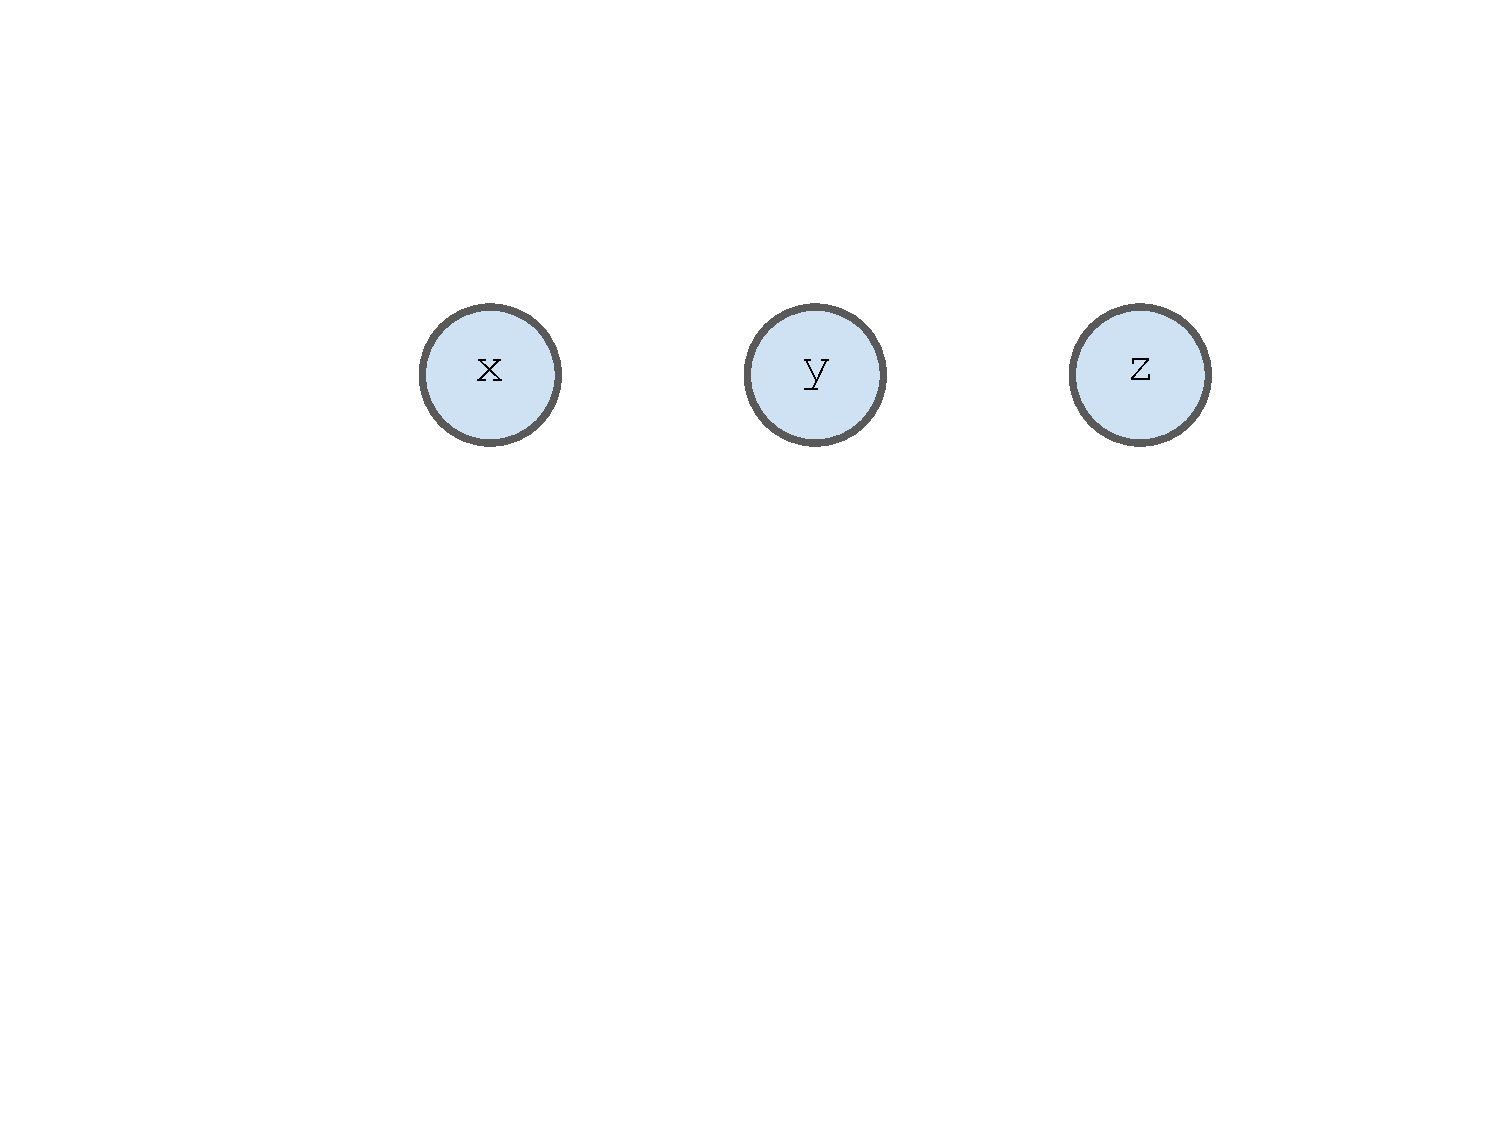
\includegraphics[trim={35mm 115mm 35mm 51mm},clip,width=0.8\linewidth]{alias-graph0.pdf}
%%  \end{minipage}
%%%  \caption{Example alias graph data structure.}
%%%    \label{fig/alias-graph}
%%\end{figure}
%%
%%Aliasing can be induced by various program operations (e.g.,
%%\relname{Move}, \relname{Load}, and \relname{Store}), as seen in
%%our earlier model. Since we are interested in must-alias, two
%%aliased variables have to point to the same object---their nodes
%%can be merged if a \relname{Move} instruction, \code{x = y}, is
%%encountered:
%%
%%\begin{figure}[h]
%%  \begin{minipage}[b]{\linewidth}
%%    \centering
%%    % left bottom right top
%%    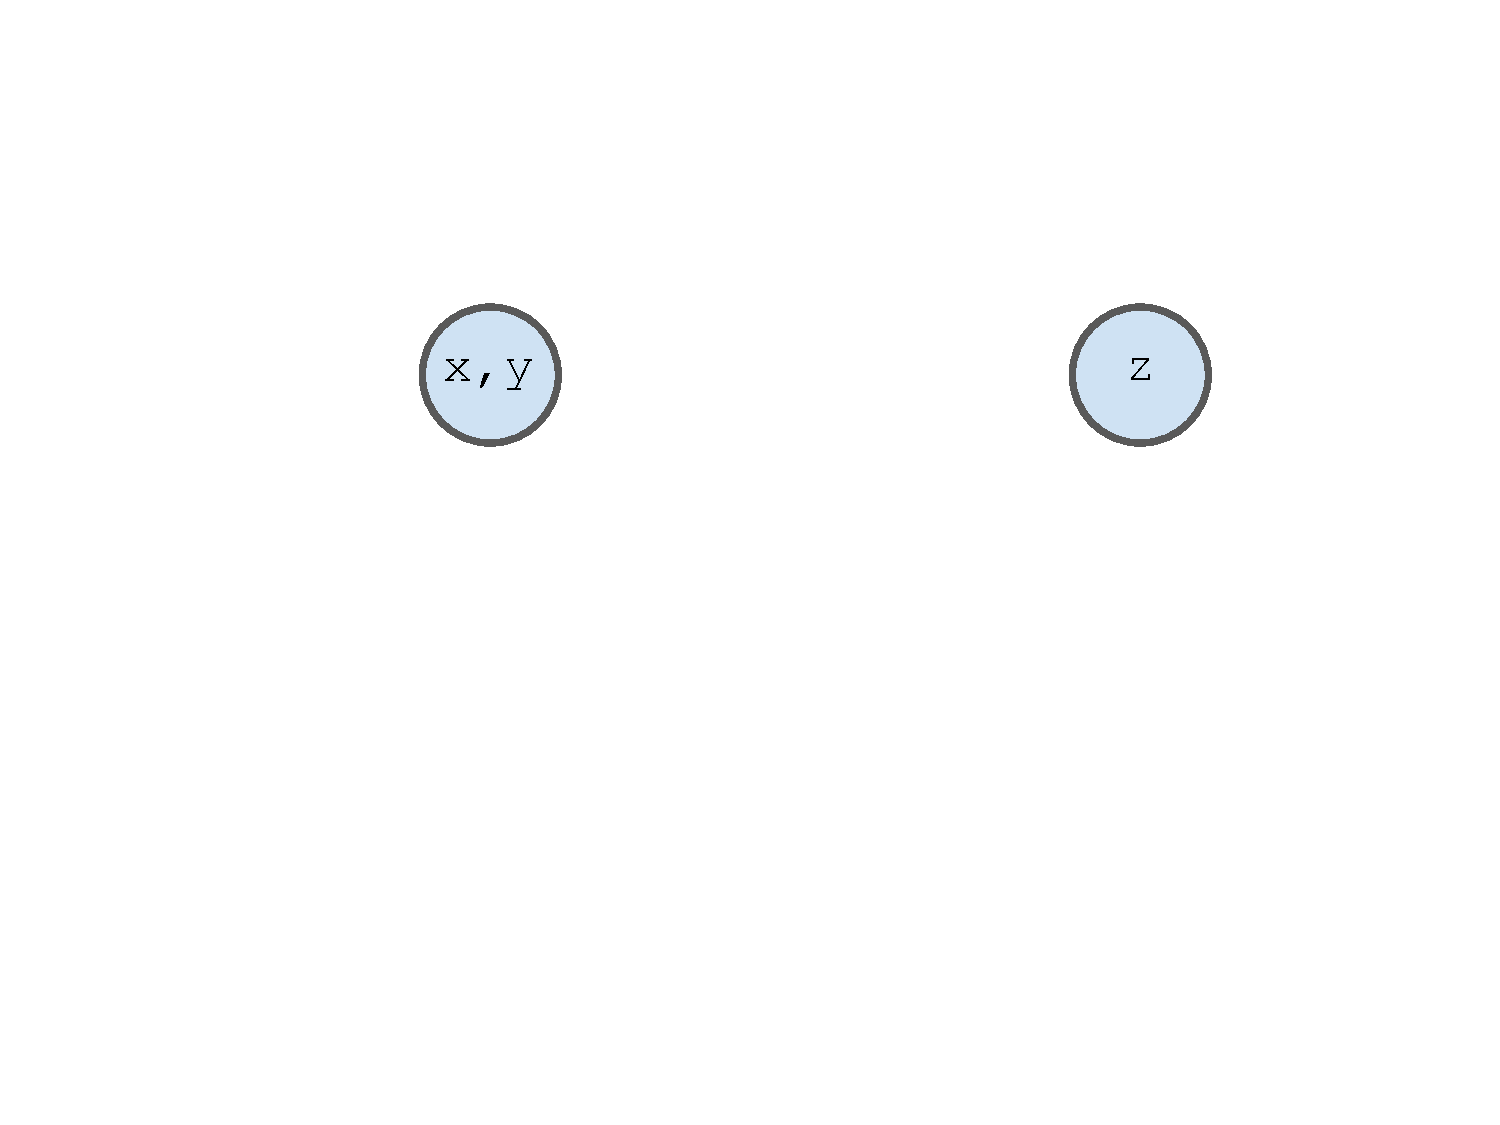
\includegraphics[trim={35mm 115mm 35mm 51mm},clip,width=0.8\linewidth]{alias-graph1.pdf}
%%  \end{minipage}
%%%  \caption{Example alias graph data structure.}
%%%    \label{fig/alias-graph}
%%\end{figure}
%%
%%%That is, the new graph \emph{after} the \relname{Move} instruction will
%%%contain the collapsed node.
%%
%%If the next instruction is a \relname{Store}, \code{x.f = z}, the
%%previous graph will get propagated. Subsequently, the \relname{Store}
%%will add an edge to the graph, signifying that the field, \code{f}, of
%%the object pointed by \code{x} will point to the object that \code{z}
%%points to:
%%
%%\begin{figure}[h]
%%  \begin{minipage}[b]{\linewidth}
%%    \centering
%%    % left bottom right top
%%    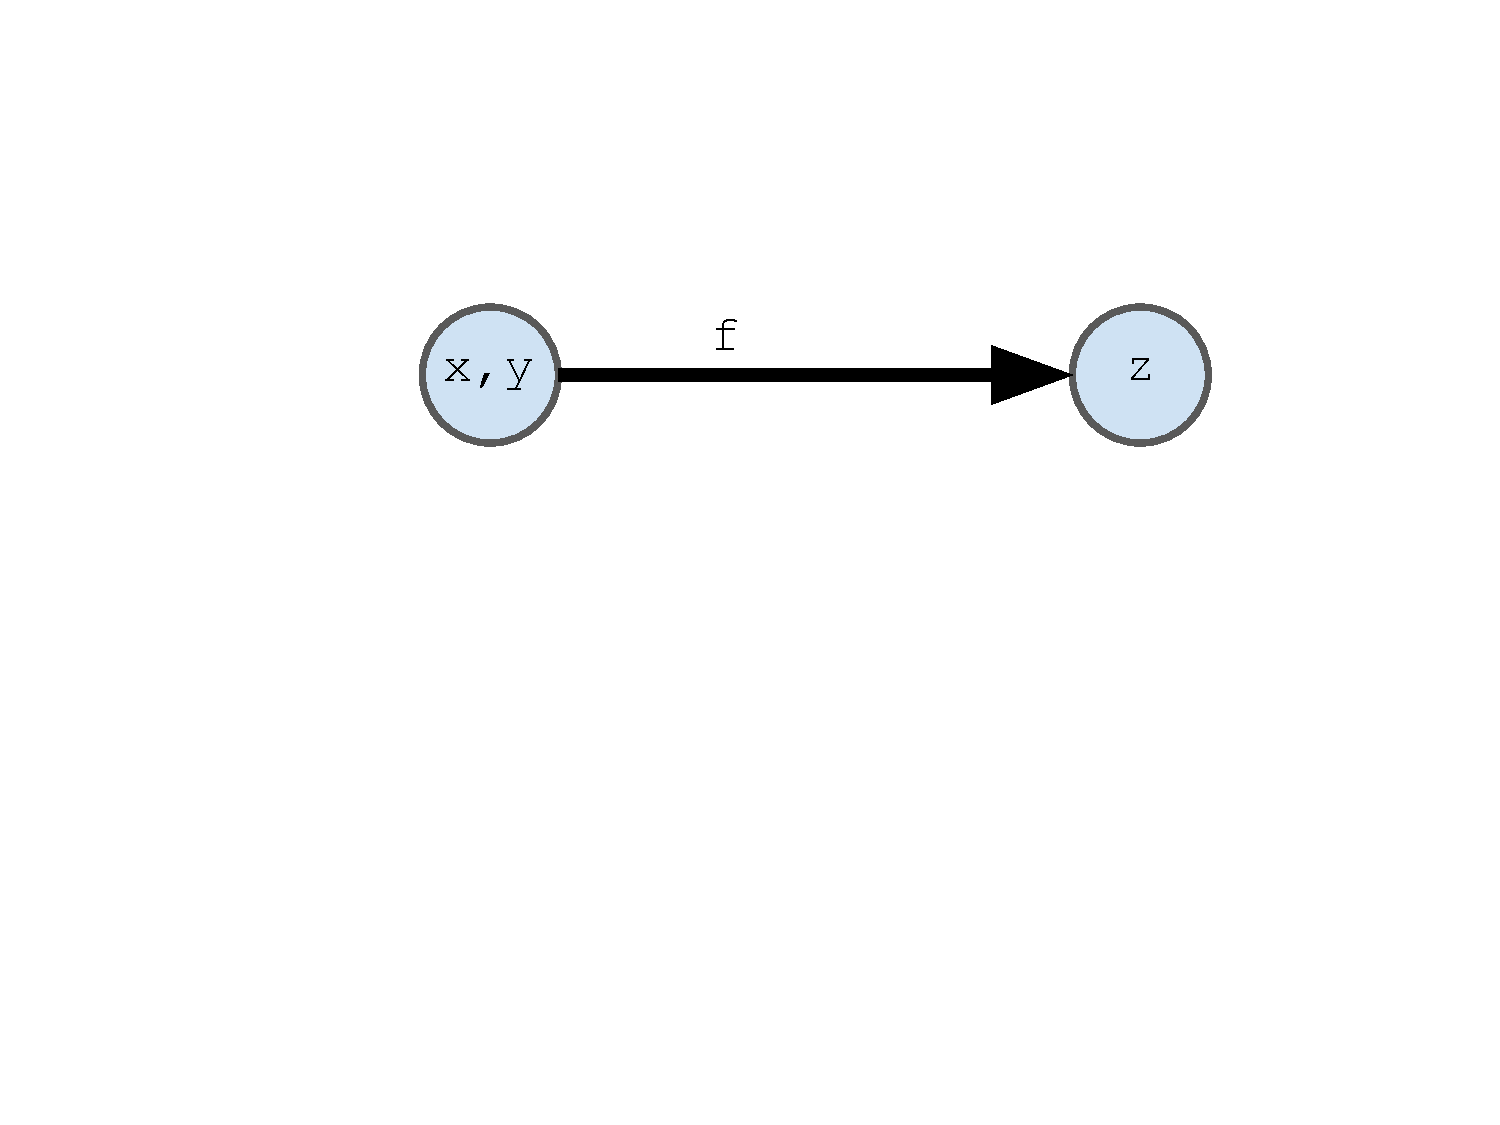
\includegraphics[trim={35mm 115mm 35mm 51mm},clip,width=0.8\linewidth]{alias-graph2.pdf}
%%  \end{minipage}
%%%  \caption{Example alias graph data structure.}
%%%    \label{fig/alias-graph}
%%\end{figure}
%%
%%A subsequent \relname{Load} operation, \code{z =
%%  y.g},\footnote{Strictly speaking, this exact scenario will never arise for
%%  our SSA input, since \texttt{z} has had its value read earlier and its
%%  single assignment has to dominate its use.}
%%will inherit the alias graph of its predecessor and will modify it.
%%Variable \code{z} is removed from its old node (\code{z} no longer points
%%to this abstract object), a new node for \code{z} is created, and the
%%nodes are linked, to indicate that \code{z} now points to the same
%%object as \code{y.g}. The empty, former node of \code{z} will be garbage
%%collected if no other paths can reach it in the alias graph.
%%
%%%https://docs.google.com/presentation/d/1FKZpmf509xiwTNGIhyaOYmo8KUsQ82zJIlc5_PQrqHI/edit#slide=id.p
%%
%%\begin{figure}[h]
%%  \begin{minipage}[b]{\linewidth}
%%    \centering
%%    % left bottom right top
%%    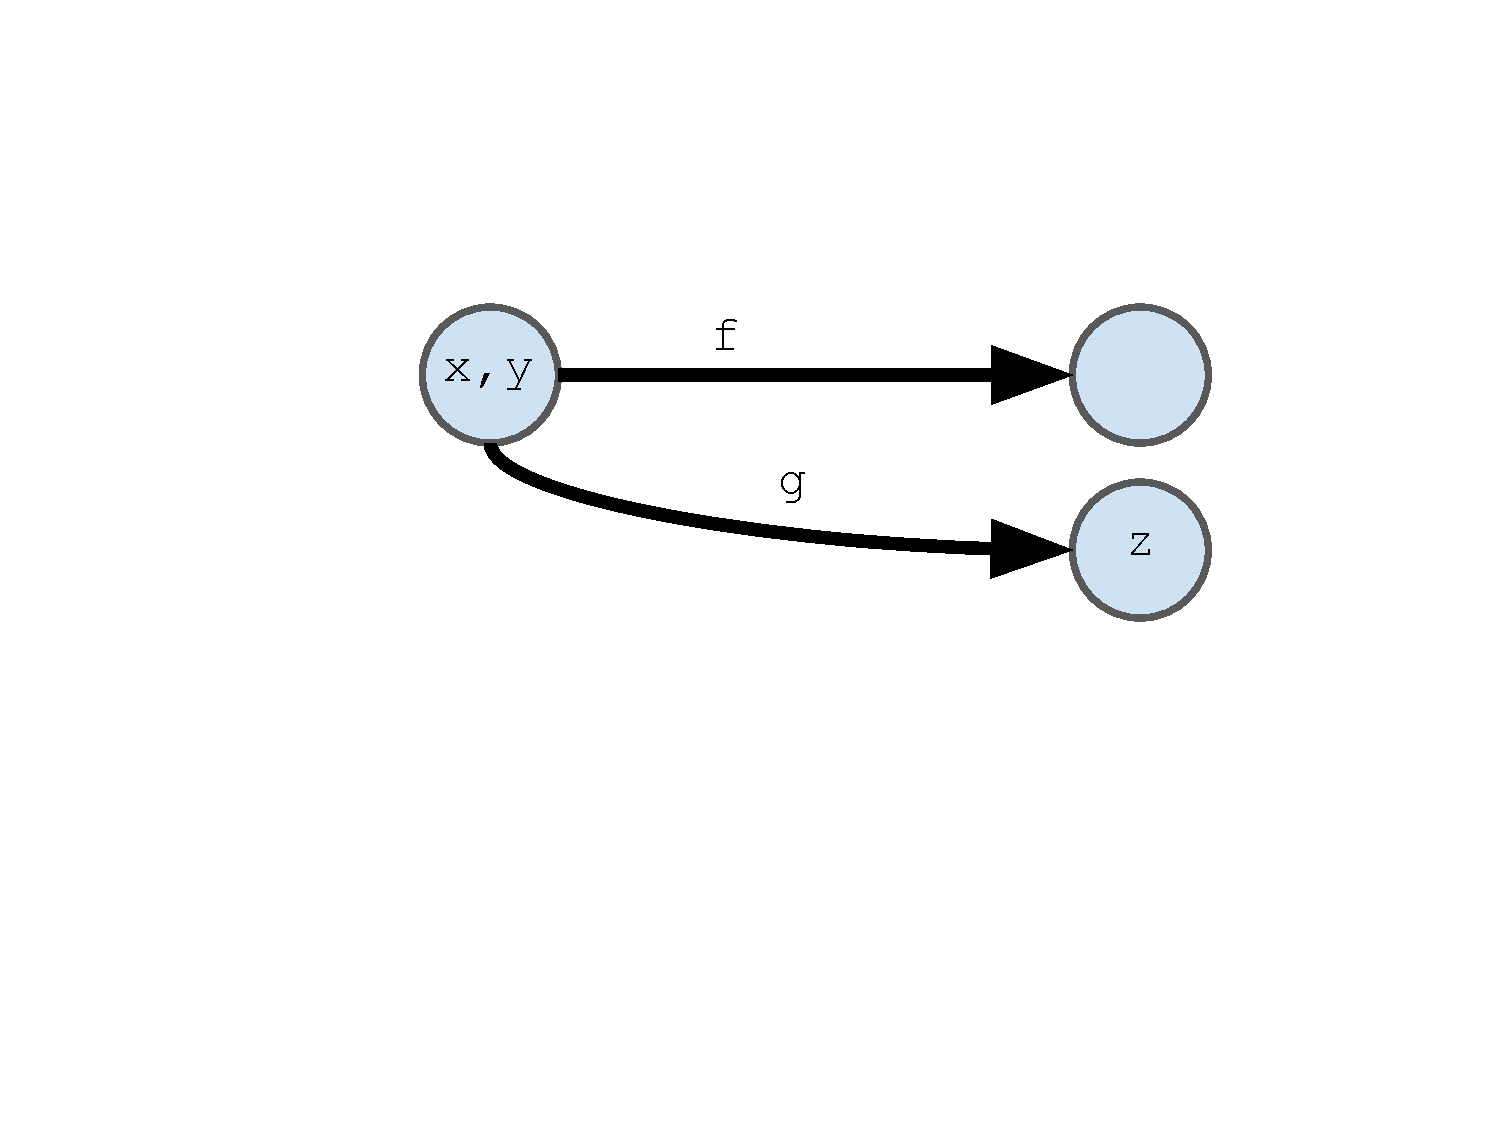
\includegraphics[trim={35mm 85mm 35mm 51mm},clip,width=0.8\linewidth]{alias-graph3.pdf}
%%  \end{minipage}
%%%  \caption{Example alias graph data structure.}
%%%    \label{fig/alias-graph}
%%\end{figure}
%%
%%The \relname{Load} operation shows that our alias graph, although
%%intended to abstractly represent a real heap, behaves quite
%%differently: a load from a field can introduce new objects, as well as
%%update fields of existing objects.
%%
%%Generally, the alias graph captures compactly all aliasing
%%relationships among access paths. Maintaining the graph across program
%%instructions is simple, as in the above examples. Graph manipulation
%%merely has to observe some invariants:
%%
%%\begin{itemize}
%%  \item Two variables are in the same graph
%%node iff they are aliased. (Since alias classes are disjoint, the
%%variables in different nodes are also disjoint.)
%%  \item A path in the graph
%%represents a set of access paths, starting from a non-empty node (that
%%denotes the base variables of the access paths) and extended with the
%%field labels along the path's edges. If two paths in the graph reach
%%    the same node, all access paths they represent must be aliased.
%%\end{itemize}
%%
%%For
%%illustration, consider Figure~\ref{fig/alias-graph}, which shows the
%%alias graph after line 31 of our example in Section~\ref{sec:example}.
%%
%%%https://docs.google.com/drawings/d/1eJQXf-azf7oXZpeu-RQTpfcaGDbnigINMnHQJ8CKUWg/edit?usp=sharing
%%
%%\begin{figure}[h]
%%  \begin{minipage}[b]{\linewidth}
%%    \centering
%%    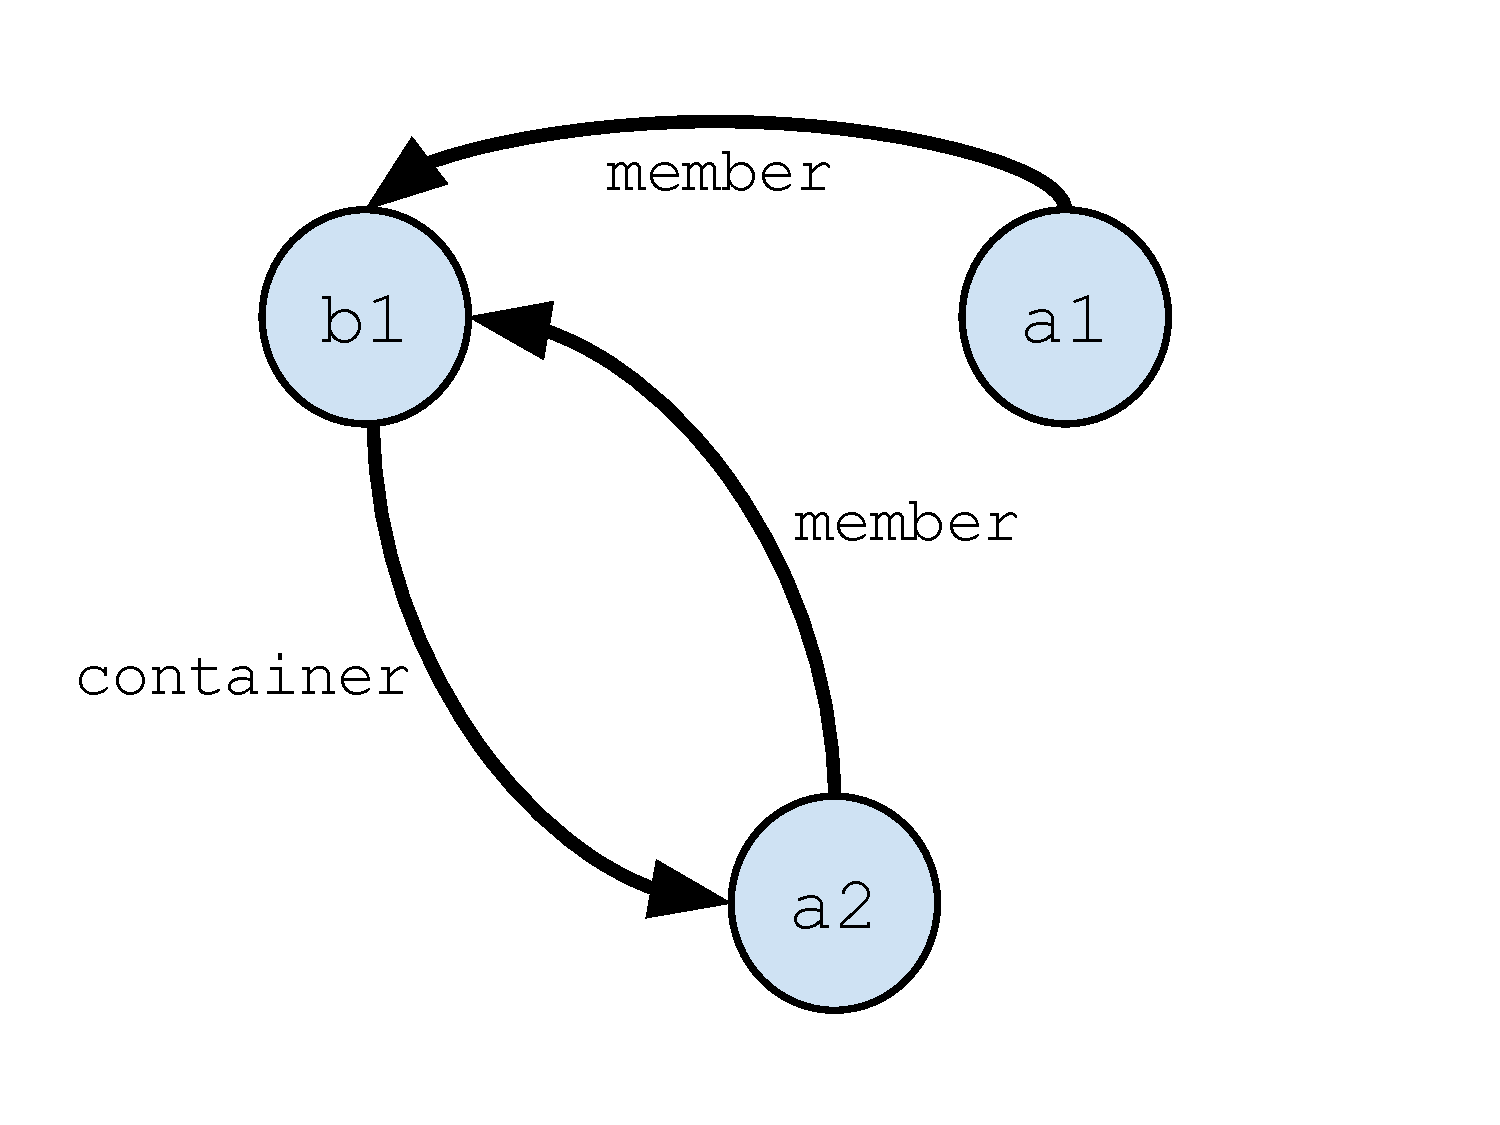
\includegraphics[trim={13mm 15mm 10mm 10mm},clip,width=0.7\linewidth]{alias-graph.pdf}
%%  \end{minipage}
%%  \caption{Example alias graph data structure.}
%%    \label{fig/alias-graph}
%%\end{figure}
%%
%%The graph concisely represents a set of alias relationships that hold
%%at that program point: \code{b1.container} $\sim$ \code{a2},
%%\code{a1.member} $\sim$ \code{b1}, and \code{a2.member} $\sim$ \code{b1}. An
%%infinite number of other alias pairs are represented implicitly:
%%\code{a1.member} $\sim$ \code{a2.member}, \code{a1.member.container} $\sim$
%%\code{a2}, \code{a1.member.container.member} $\sim$ \code{b1},
%%\code{a1.member.container.member} $\sim$ \code{a1.member}, etc.
%%
%%Overall, the alias graph satisfies both of our requirements of
%%Section~\ref{sec:needs} for an efficient representation.  Equivalence
%%relations are represented compactly: an alias class with $n$ members
%%does not need $n^2$ space and time for its computation.  Instead,
%%it is represented implicitly, as all the alias graph paths that can
%%reach a node. (In the case of aliased variables, the representation is
%%immediate, since they belong in the same node.) Similarly, long (and
%%even infinite) access paths are represented implicitly as graph paths.
%%
%%
%%%A node recursively represents an alias set: that of all
%%%paths in the graph that reach it. A node $n_1$ has an edge labeled $f$
%%%to a node $n_2$ iff the access paths represented by $n_1$
%%
%%
%%\subsection{Main Algorithms}
%%
%%Most of the required must-alias analysis actions (per the model of
%%Section~\ref{sec:model}) over our data structure are
%%straightforward, consisting of copying, additions and removals of
%%variables and edges, and variable renamings. Standard mappings for efficient
%%indexing are required: each target of a directed edge needs to be able
%%to quickly retrieve its source, and each program variable needs to
%%quickly map to the node in which it appears. 
%%
%%For instance, according to the earlier definition of the data
%%structure, finding all aliases of an access path is simple (but requires a
%%transitive computation---our graph is a condensed representation of alias
%%classes):
%%
%%\paragraph{Algorithm: \code{all-aliases(ap)}}
%%\begin{itemize}
%%\item Find the node for the base variable of access path \code{ap}, traverse
%%   in the forward direction the labeled edges that match each of the fields
%%   of \code{ap} to reach a target node.
%%\item Any graph path that reaches the same node corresponds to an
%%  aliased access path, from a base variable adding the fields
%%  labeling the edges. (I.e., traverse $k-1$ directed edges backwards
%%  to find access paths of length up to $k$.)
%%\end{itemize}
%%
%%For instance, in Figure~\ref{fig/alias-graph}, we can find all aliases
%%of length 3 of access path \code{a2.member} by traversing edge
%%\code{member} from node \code{a2} (thus reaching the node containing
%%\code{b1}) and finding all paths of length 2 that can reach the same
%%node, also including the variable(s) in the starting node of the path
%%(e.g., \code{b1.container.member}).
%%
%%The more interesting algorithm, as suggested earlier, is that of
%%intersecting alias graphs---necessary for merging alias information
%%from predecessor instructions. This is easy to see as a repeated
%%intersection of two graphs (which is then iterated by intersecting a
%%third with the result, then a fourth, and so on). Note that the graphs
%%do not need to contain a single connected component.
%%
%%\paragraph{Algorithm: \code{intersect($g_1$,$g_2$)}}
%%\begin{itemize}
%%\item For every two nodes $i$, $j$ of $g_1$ and $g_2$, respectively, create new node $(i,j)$.
%%    Its variables are the intersection of the variables of $i$ and $j$.
%%\item For every label $f$, if $g_1$ has an edge $i \rightarrow k$ with
%%  label $f$, and $g_2$ has an edge $j \rightarrow l$, also with label $f$, the
%%   intersection result has an edge $(i,j) \rightarrow (k,l)$ with label $f$.
%%\end{itemize}
%%
%%The algorithm considers all possible pair-wise node combinations and
%%all possible edges out of node intersections. 
%%
%%Notably, the intersection of two alias graphs can produce nodes with
%%empty variable sets. To illustrate, consider the example in
%%Figure~\ref{fig/intersection}.
%%
%%%https://docs.google.com/drawings/d/1gi-CsxoOFJ9E99KF4e8kgzqcDMjBOUcwObCXV8sVQyU/edit?usp=sharing
%%
%%\begin{figure}[h]
%%  \begin{minipage}[b]{\linewidth}
%%    \centering
%%    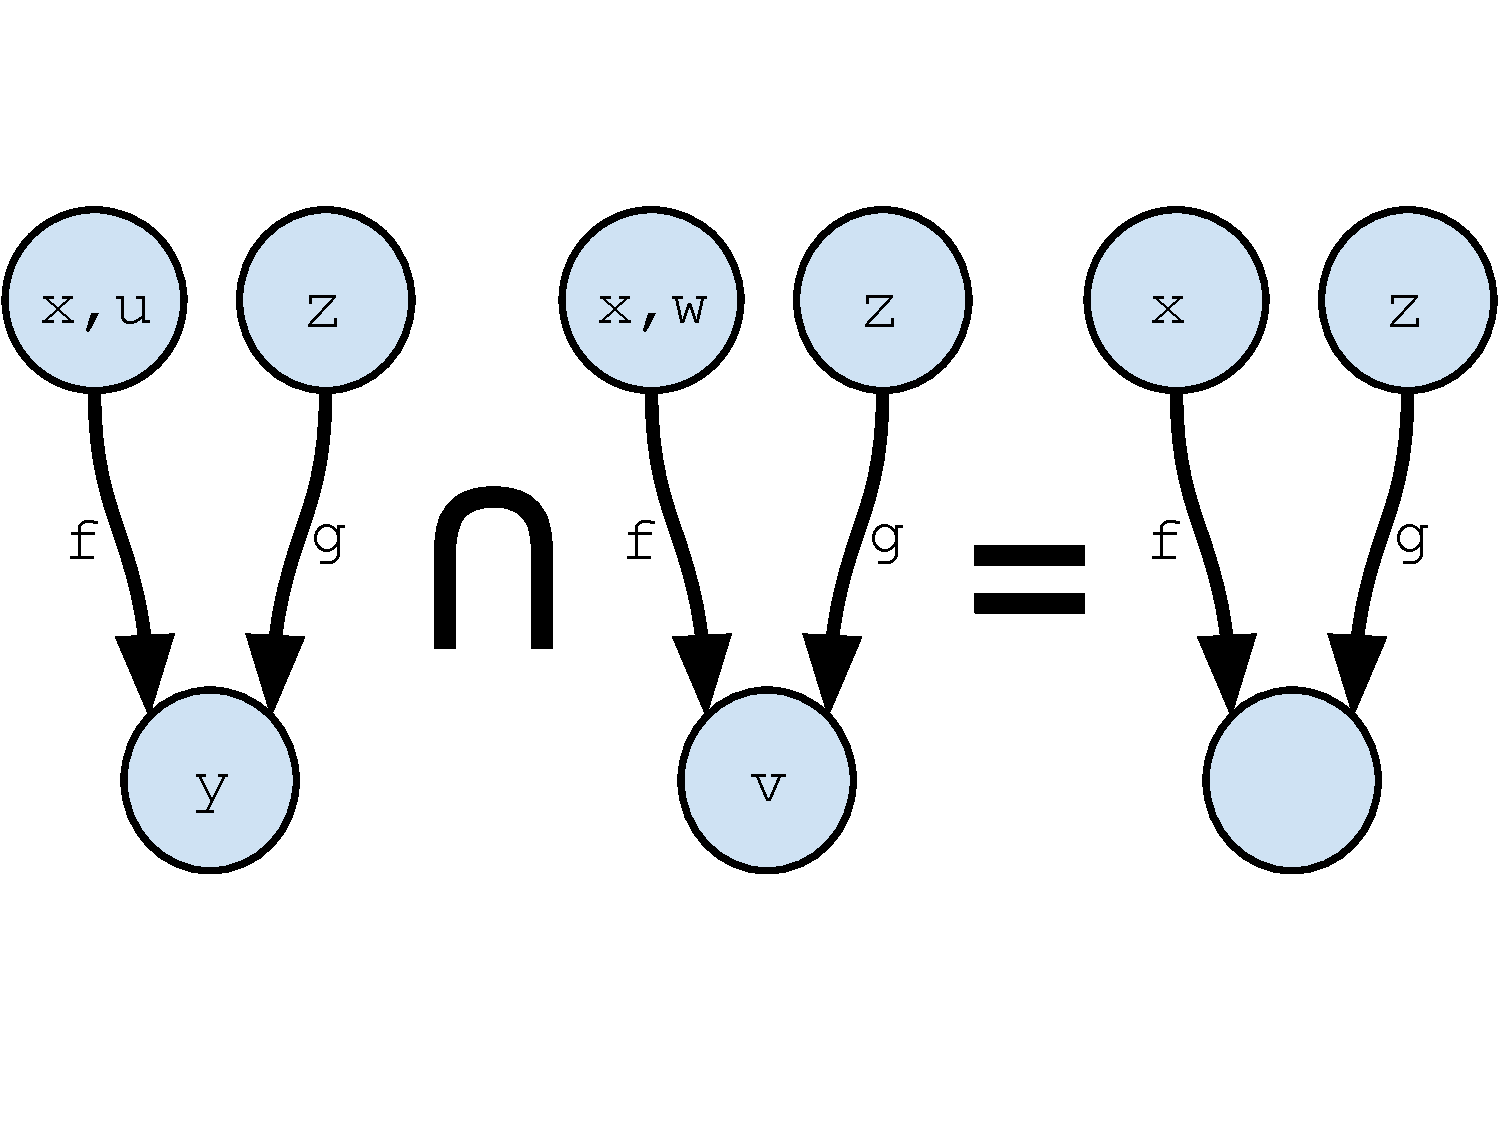
\includegraphics[trim={0mm 40mm 0mm 30mm},clip,width=0.9\linewidth]{intersecting-alias-graphs.pdf}
%%  \end{minipage}
%%  \caption{Intersecting alias graphs}
%%    \label{fig/intersection}
%%\end{figure}
%%
%%In this case, the empty note denotes that access paths \code{x.f} and
%%\code{z.g} are still aliased in the intersection alias graph, even
%%though they are no longer aliased with any single-variable access
%%path.
%%
%%For upper bounds $n$, $m$, $v$, $e$ in the number of nodes, empty nodes,
%%variables, and edges per alias graph, respectively, the
%%algorithm has a running time asymptotic bound of $O(nm + v + e)$,
%%i.e., linear in all quantities except nodes when many are empty, if
%%one assumes a practically constant-time indexing scheme from a
%%variable to its node. (Proof sketch: Non-empty nodes are fewer than
%%variables and only linear cost is incurred when combining non-empty
%%nodes pair-wise, since each node has a distinct set of variables, used
%%to index into any node that may intersect that set in the other alias
%%graph. In contrast, empty nodes have a trivial, empty, intersection
%%set of variables, but need to be examined in all pair-wise
%%combinations with other nodes to find matching edges.) 
%%Empty nodes are expected to arise rarely in practice.
%%
%%Other simple algorithmic enhancements apply to our data structure. For
%%instance, nodes should be garbage-collected for maximum efficiency, if
%%they stop encoding access path aliasing. The node collection algorithm
%%is as follows:
%%
%%\paragraph{Algorithm: \code{gc($g$)}}
%%\begin{itemize}
%%\item Any node in $g$ containing a single variable and with no incoming or outgoing
%%  edges is eliminated.
%%\item Any node in $g$ containing no variables and with either zero in-edges
%%  or one in-edge and zero out-edges is eliminated.
%%\end{itemize}
%%
%%
%%\subsection{Declarative Implementation}
%%
%%As discussed earlier, the alias graph data structure can be employed
%%in a must-alias analysis by maintaining alias graphs per-program-point
%%(i.e., per context-qualified instruction), and updating them (to
%%incorporate information from their predecessor instructions) until
%%fixpoint.
%%
%%The data structure description we have seen so far considers this
%%update to be a destructive operation. For instance, after a
%%\relname{Move} instruction, we saw the nodes of two variables getting
%%merged. Similar merging can be induced by information that the
%%analysis discovers while it is executing (i.e., not directly induced
%%by the semantics of the current instruction)---e.g., propagated from
%%predecessors.
%%
%%We have also designed and implemented a declarative/purely functional
%%version of the data structure. The main reason for the declarative
%%implementation has been fairness in experimental comparisons. We will
%%compare our optimized implementation against the must-alias analysis
%%of the \textsc{Doop} framework, implemented in Datalog. Thus, it is desirable
%%to also implement a, perhaps not as optimal, declarative version of
%%the data structure in Datalog. This will allow us to isolate the
%%effect of destructive updates from the inherent properties of the data
%%structure.
%%
%%In the declarative version of the structure, aliased abstract objects
%%are not merged, but instead associated with each other. Schematically,
%%we can consider that each variable has its own node and points to
%%at least one abstract object---at first the abstract object signifying
%%``whichever object the variable got assigned to'' (at its single-assignment
%%site):
%%
%%%Thus, nodes of the graph
%%%are either variables or object abstractions, and edges correspond to
%%%variable-points-to (edge from variable to object) and
%%%object-field-points-to (edge from object to object) relationships.
%%
%%\begin{figure}[h]
%%  \begin{minipage}[b]{\linewidth}
%%    \centering
%%    % left bottom right top
%%    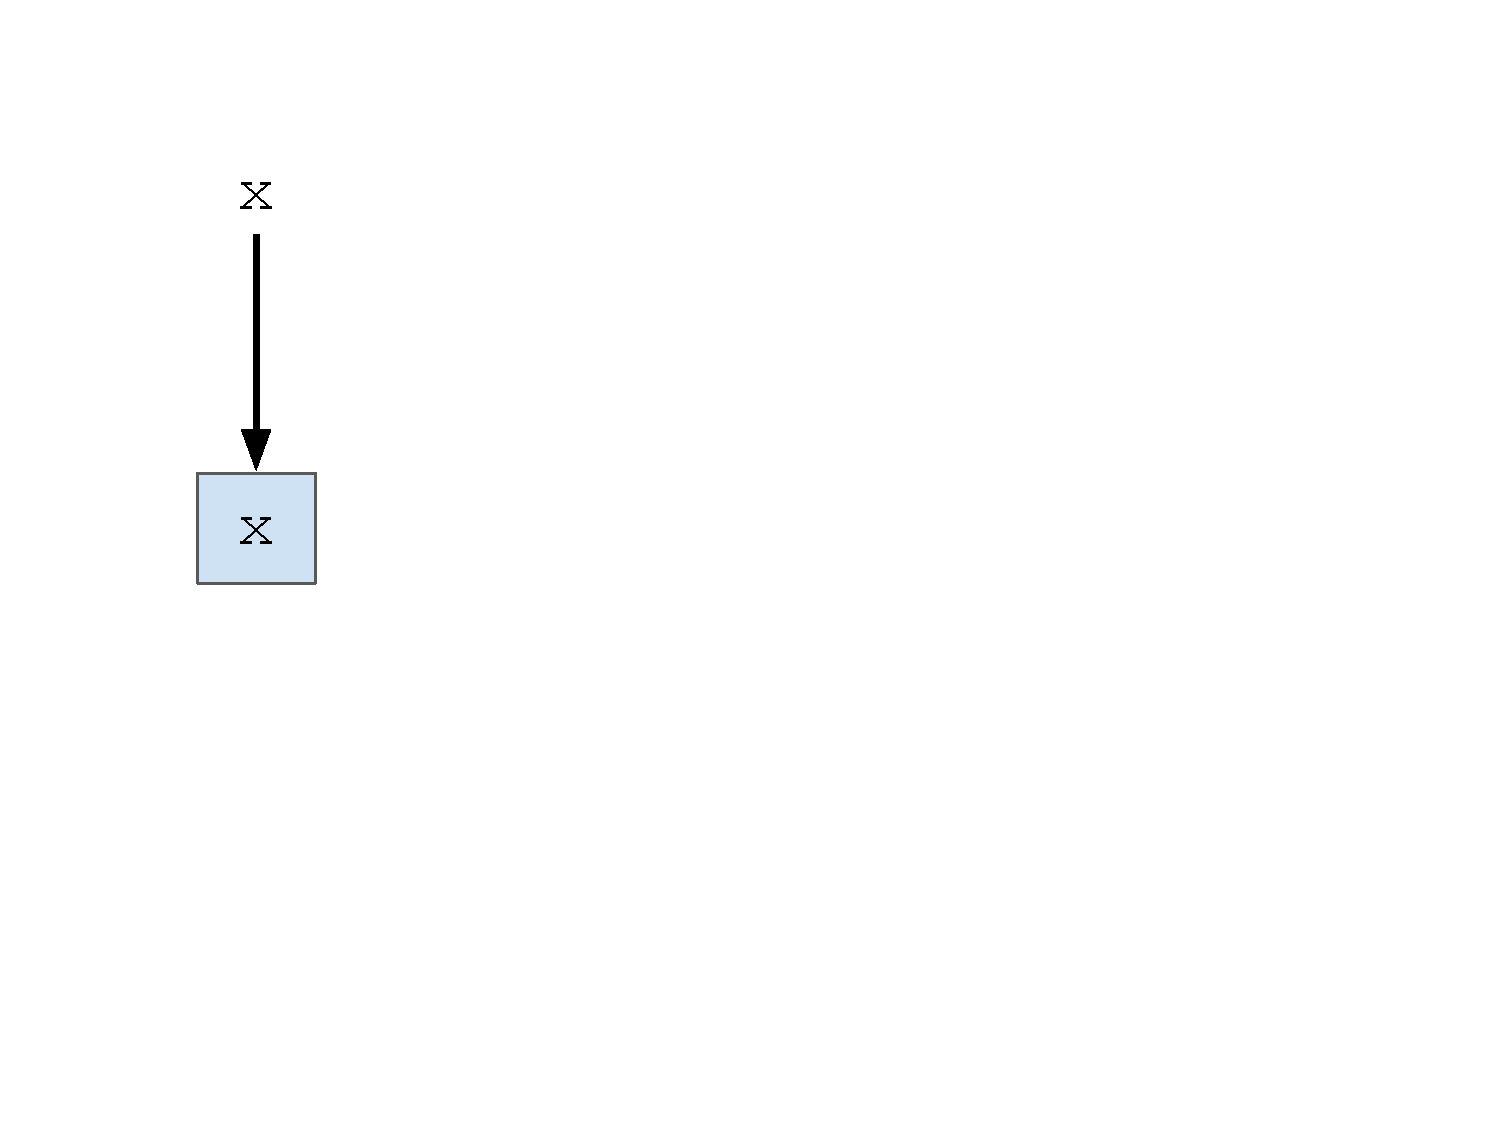
\includegraphics[trim={25mm 90mm 190mm 25mm},clip,width=0.15\linewidth]{decl-alias-graph0.pdf}
%%  \end{minipage}
%%%  \caption{Example alias graph data structure.}
%%%    \label{fig/alias-graph}
%%\end{figure}
%%
%%(For the declarative implementation, we will represent abstract objects
%%as squares, to avoid confusion.)
%%
%%Since we no longer have destructive updates, variables can point
%%to multiple abstract objects. For instance, after a \relname{Move} instruction,
%%\code{x = y}, we have:
%%
%%%\begin{figure}[h]
%%  \begin{minipage}[b]{\linewidth}
%%    \centering
%%    % left bottom right top
%%    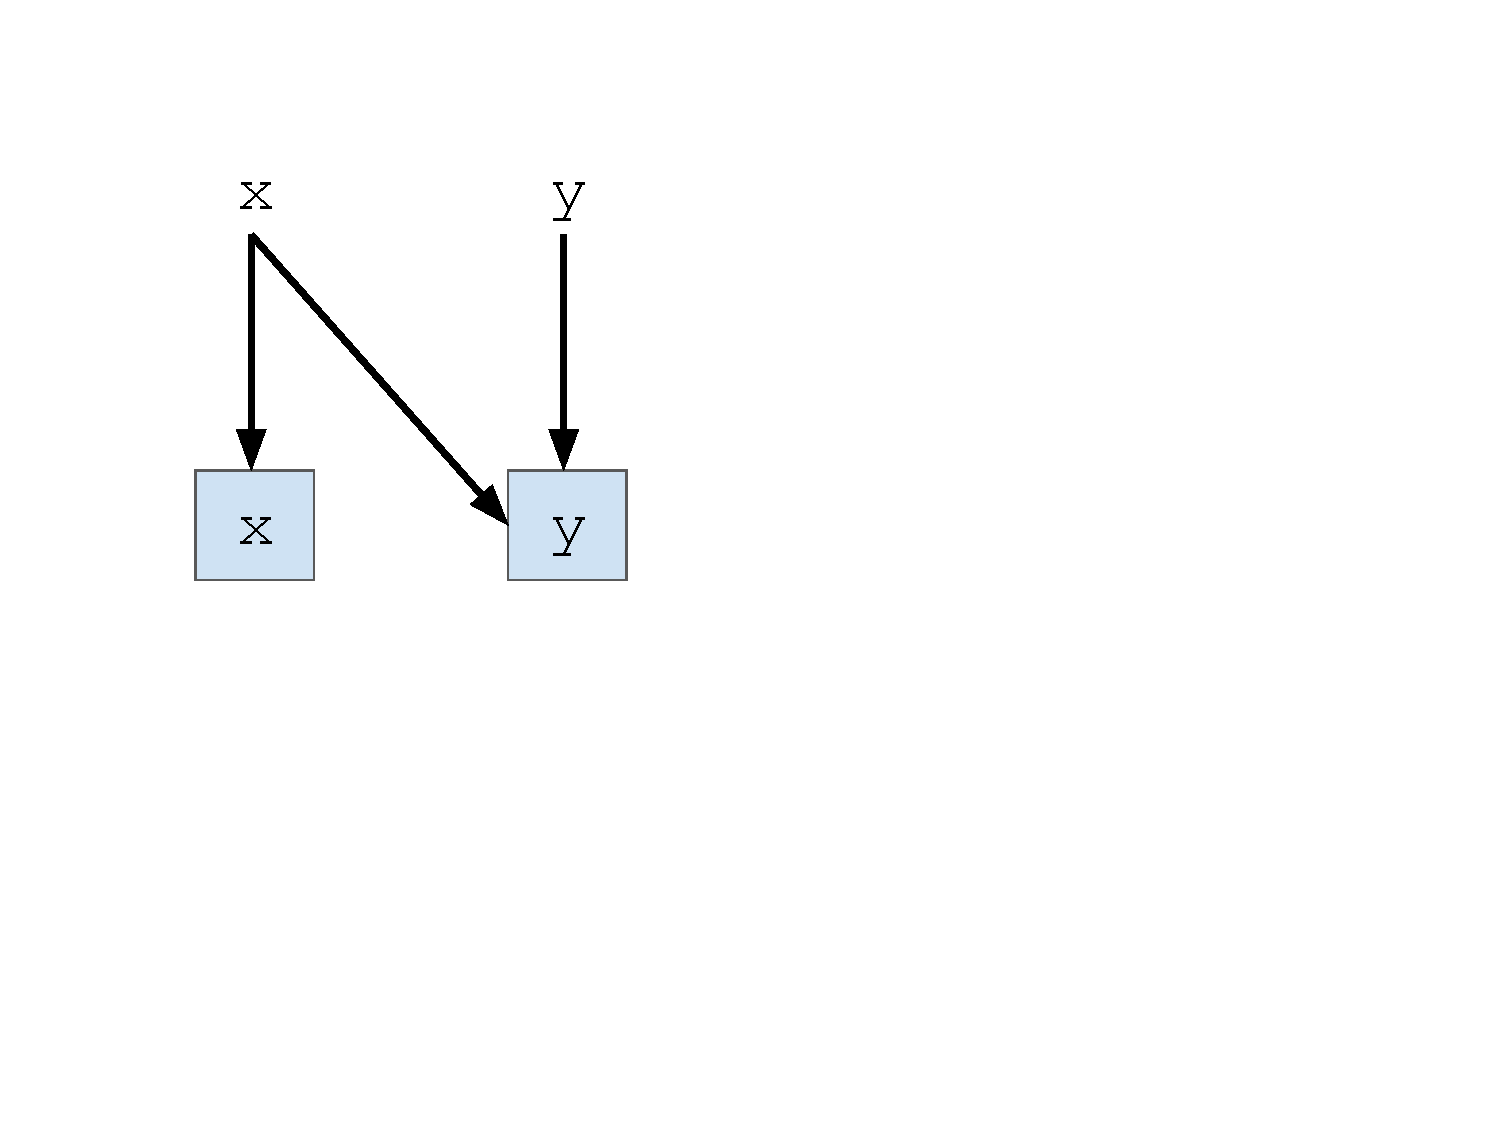
\includegraphics[trim={30mm 90mm 140mm 25mm},clip,width=0.32\linewidth]{decl-alias-graph1.pdf}
%%  \end{minipage}
%%%  \caption{Example alias graph data structure.}
%%%    \label{fig/alias-graph}
%%%\end{figure}
%%
%%As before, however, a variable can really point to a single concrete
%%object. Therefore, the two abstract objects that \code{x} points to have
%%to be different abstractions of the same concrete object---their
%%equivalence is encoded, but implicitly. It is easy to check that
%%variables \code{x} and \code{y} are aliased, in the usual sense: they both
%%point to the same abstract object.
%%
%%If the next operation is another \relname{Move}, \code{z = x}, variable
%%\code{z} is made to point to both abstract objects that \code{x} points to:
%%
%%\begin{figure}[h]
%%  \begin{minipage}[b]{\linewidth}
%%    \centering
%%    % left bottom right top
%%    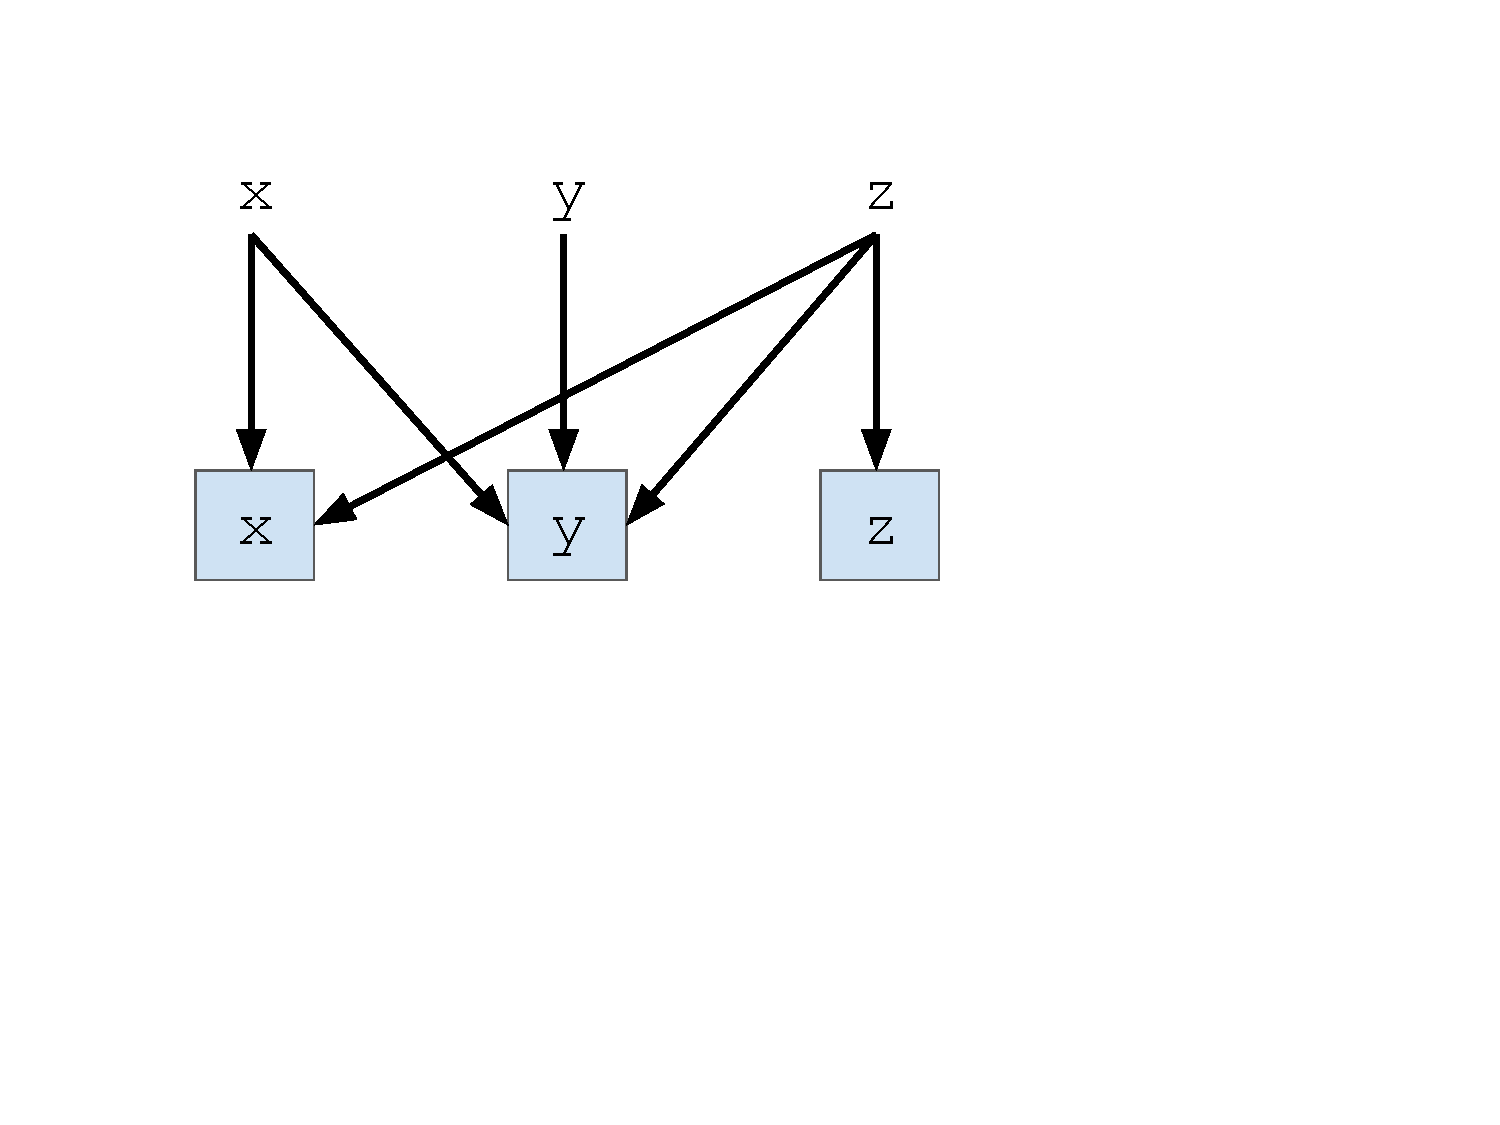
\includegraphics[trim={25mm 85mm 70mm 25mm},clip,width=0.6\linewidth]{decl-alias-graph2.pdf}
%%  \end{minipage}
%%%  \caption{Example alias graph data structure.}
%%%    \label{fig/alias-graph}
%%\end{figure}
%%
%%Thus, the declarative data structure is less efficient than its
%%imperative counterpart: a quadratic representation of an alias set
%%cannot be precluded, and depends on the order of alias-inducing
%%instructions. In our example, we could then assign \code{z}, the
%%variable with the most out-edges, to a new variable, \code{w}, then
%%assign \code{w} (which now has the most out-edges) to a new variable,
%%and so on.  In practice we expect that this effect will be mitigated.
%%If the next instruction assigns \code{y} to a new variable, \code{u}, then
%%\code{u} receives only a single extra edge, maintaining a more compact
%%representation of the alias set. The cost, much as in the imperative
%%structure, is that the alias set is not fully explicit and requires a
%%transitive closure computation to be materialized.
%%
%%
%%
%%%% Intuitively, the key element of our data structure is the introduction
%%%% of a different kind of abstract object. In traditional analyses, an
%%%% abstract object represents multiple concrete objects.  In our setting,
%%%% we introduce abstract objects that represent \emph{at most one}
%%%% concrete object. Abstract objects correspond to variables and are a
%%%% symbol for the concept ``the object that the variable points to''.
%%%% When a variable is inferred to point to an abstract object, the
%%%% variable \emph{must} point to a matching object at that
%%%% program location. In this way, we can infer (definite) aliasing
%%%% when a variable points to multiple abstract objects. For an
%%%% example, consider the configuration below:
%%
%%%% \begin{figure}[h]
%%%%   \begin{minipage}[b]{\linewidth}
%%%%     \centering
%%%%     % left bottom right top
%%%%     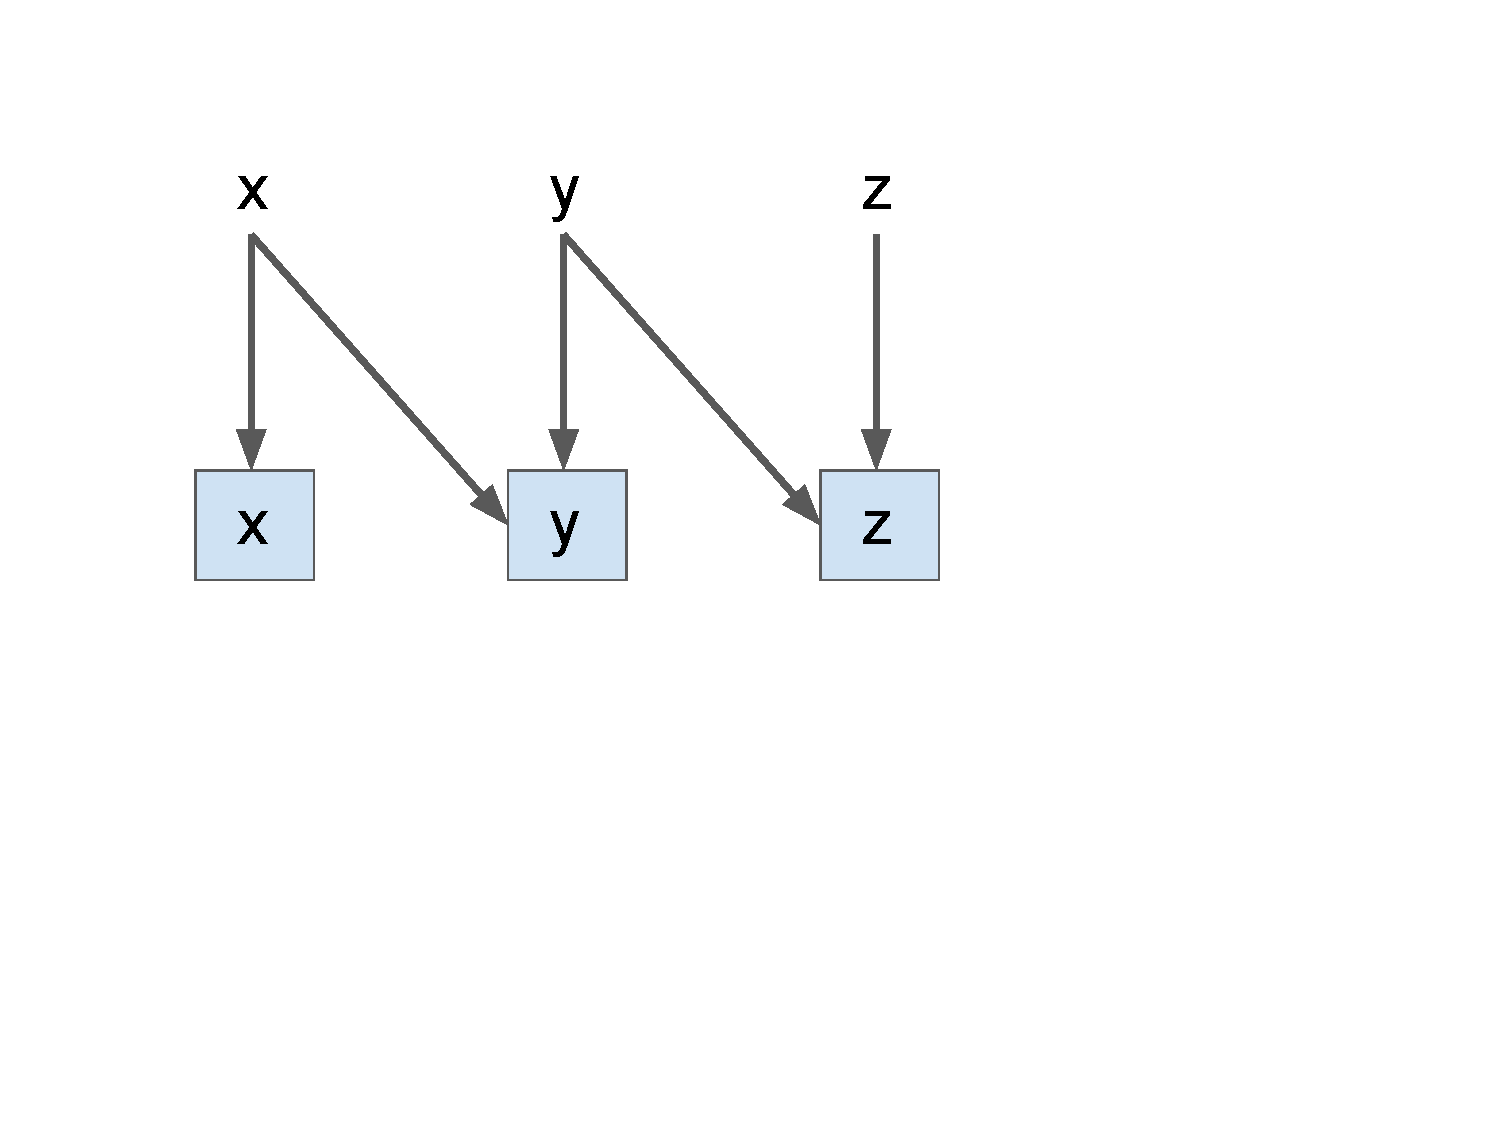
\includegraphics[trim={25mm 85mm 70mm 25mm},clip,width=0.5\linewidth]{alias-intro2.pdf}
%%%%   \end{minipage}
%%%% %  \caption{Example alias graph data structure.}
%%%% %    \label{fig/alias-graph}
%%%% \end{figure}
%%
%%%% Since variable \code{x} must point to two abstract objects, they have to
%%%% correspond to the same run-time object. That is, the object that
%%%% variable \code{x} points to has to be the same as the object that
%%%% variable \code{y} points to. This is hardly surprising, since the figure
%%%% clearly shows the two variables point to a common object.  However,
%%%% variable \code{y} also points to two abstract objects, thus the two need
%%%% to represent the same concrete object. Therefore, \code{y} and \code{z}
%%%% are aliased, and so are \code{x} and \code{z}: all three variables are in
%%%% the same must-alias set. In a basic sense, this is the kind of
%%%% reasoning that our data structure encodes, to represent aliasing
%%%% compactly, for arbitrarily deeply nested structures.



%% \section{Implementation and Experiments}
%% \label{sec:experiments}
%% 
%% As already mentioned, the analysis model of Section~\ref{sec:model} corresponds
%% closely to the must-alias analysis implementation in the \textsc{Doop}
%% framework for Java bytecode analysis. We aim to improve over this direct
%% encoding of the must-alias relation. We implemented the analysis in Java, to
%% evaluate our optimized (imperative) alias graph data structure. Finally, we
%% implemented an optimized Datalog implementation, based on our purely functional
%% data structure.
%% 
%% %of Section~\ref{sec:datastructure}.
%% The three implementations are functionally equivalent, with very minor
%% variations, due to clear engineering differences: The original Datalog analysis
%% has to bound the access path length for aliases to a finite number, while the
%% optimized data structure implicitly stores aliases for longer access paths.
%% %% This may allow inferring more aliases even for shorter access paths. Also, for engineering simplicity, the
%% %% Java implementation incorporates just a naive fixpoint computation.
%% %% In each fixpoint iteration, it keeps track of a set of instructions whose
%% %% alias graphs might be affected by the current changes, and those are
%% %% the instructions that will be inspected in the next iteration. This process
%% %% is repeated until there are no further instructions for consideration.
%% %% The fixpoint computation is only crudely tuned for performance and
%% %% the algorithm is eager to mark an instruction as a candidate for the next iteration.
%% 
%% %% Since the analyses are virtually equivalent, we next compare them only
%% %% on speed. (For context, however: the analysis is quite effective and computes
%% %% far from trivial results. It produces enough must-alias inferences to
%% %% determine unique points-to targets for 20-40\% of local variables in
%% %% all benchmarks. Its current main uses inside \textsc{Doop} are to
%% %% enable strong updates in a may-point-to analysis, as well as to
%% %% produce results for inspection by humans, to aid program
%% %% comprehension.)
%% 
%% We use a 64-bit machine with an Intel(R) Xeon(R) E5-2687W v4 (24-cores) CPU at
%% 3.00GHz. The machine has 512GB of RAM. All measurements are single-threaded
%% (though, as is common, Java runs its garbage collector in extra threads) and
%% all executions occupy only a small fraction of the available RAM. We experiment
%% with the DaCapo benchmark programs~\cite{oopsla:2006:Blackburn} v.2006-10-MR2 and
%% v.9.12-bach under JDK 1.7.0\_45.  We use the LogicBlox Datalog engine,
%% v.3.10.14.
%% 
%% \paragraph{Speed across benchmarks.}
%% 
%% Figure~\ref{fig:time} shows the performance effect of our optimized data
%% structure on analyzing the benchmark programs. We bounded the access path
%% length (for the original Datalog analysis) to 3 and the analysis context depth
%% to 2.
%% 
%% Note that the figure is log-scale. Across all benchmarks, the difference
%% between the optimized implementations and the original is typically at least an
%% order of magnitude and often close to two.  The speedup of the two optimized
%% implementations (vs. the original) is also shown more explicitly in
%% Figure~\ref{fig:speedup}: over half the benchmarks enjoy speedups of over 20x
%% for both the Java and the Datalog optimized implementation. The Java version of
%% the data structure achieves a median speedup of 25.7x (min. 8.4x, max. 68.9x),
%% while the Datalog version has a median speedup of 24.6x (min. 5.4x, max.
%% 47.3x).  The analysis time typically drops from over ten minutes to under half
%% a minute. 
%% 
%% 
%% %focuses on the
%% %speedup gains from deploying such a data
%% %structure. Figure~\ref{fig:pairs} gives a bird's eye view of a
%% %complexity metric for the inference process.
%% 
%% %% %a high-level as well as complexity metrics for
%% %% %the inference process. The number of access-path points-to entries
%% %% %denotes how many access path are guaranteed to point to the most recent
%% %% %abstract object allocated at a known instruction. This is a good
%% %% %metric for mapping the must-alias inference to a more readily
%% %% %consumable quantity.
%% 
%% %% \begin{figure}
%% %%   \setlength{\tabcolsep}{6pt}
%% %%   \centering
%% %%   \begin{tabular}{||l| r| r| r| r| r||}
%% %%     \toprule
%% %%     Benchmark &      optimized &      explicit & speedup & must-alias & access path         \\
%% %%               &  time (sec)    &  time (sec)   &         & \#pairs    &  must-point-to   \\
%% %%               &                &               &         &  (Ks)      &  \# entries (Ks) \\
%% %%     \midrule
%% %%     antlr     &	39 &	1000 &	25.6  &	12130 &		1969   \\ 
%% %%     bloat     &	24 &	591  &	24.6  &  9606 &	    2268   \\ 
%% %%     chart     &	38 &	1238 &	32.6  &	22089 &		3976   \\ 
%% %%     eclipse   &	22 &	561  &	25.5  &	 8973 &	    1941   \\ 
%% %%     fop       &	28 &	527  &	18.8  &	 6571  &		1897   \\ 
%% %%     hsqldb    &	22 &	493  &	22.4  &	 6429  &		1893   \\ 
%% %%     luindex   &	13 &	398  &	30.6  &	 6303  &		1901   \\ 
%% %%     lusearch  &	15 &	416  &	27.7  &	 6887  &		1911   \\ 
%% %%     pmd       &	41 &	581  &	14.2  &	 9280  &		2059   \\ 
%% %%     xalan     &	47 &	658  &	14.0  &	 9979  &		1969   \\   
%% %%     \bottomrule
%% %%   \end{tabular}
%% %%   \caption{Execution time and main complexity metrics for our analysis
%% %%     implementations, for context depth of 1 and maximum access path
%% %%     length of 2. ``Optimized'' refers to our Java-based, optimized
%% %%     alias graph structure. ``Explicit'' is the Datalog implementation,
%% %%     maintaining all alias pairs explicitly. Also shown: the number of
%% %%     alias pairs inferred, as well as the number of must-point-to
%% %%     relationships for access paths.}
%% 
%% %%   \label{fig:time}
%% %% \end{figure}
%% 
%% \begin{figure*}[h]
%%   \begin{minipage}[b]{\linewidth}
%%     \centering
%%     % left bottom right top
%%     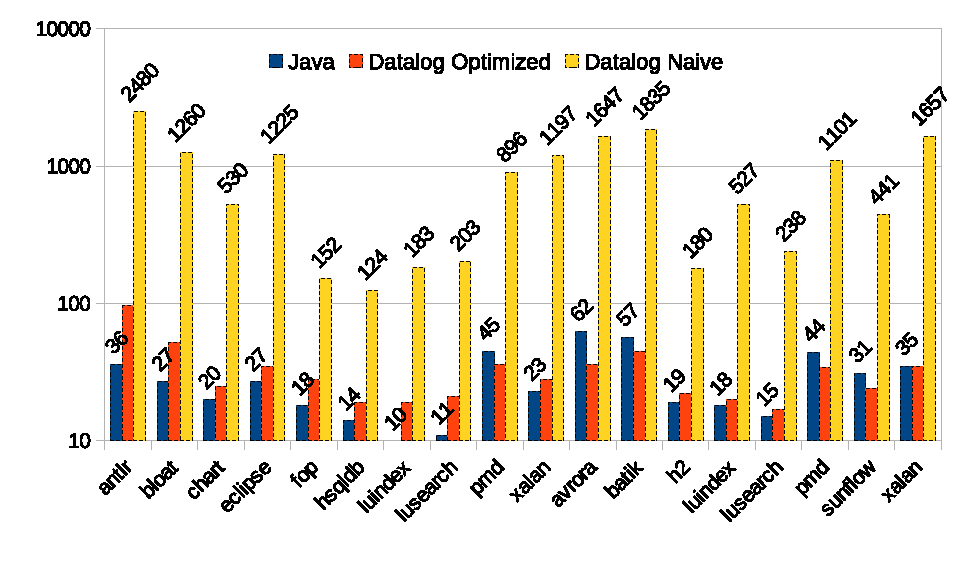
\includegraphics[clip,width=0.77\linewidth, height=0.4275\linewidth]{time.eps}
%%   \end{minipage}
%%   \caption{Execution time (sec.) of the analysis. We only show the numbers for the Java and Datalog naive versions, to avoid crowding the chart.}
%%     \label{fig:time}
%% \end{figure*}
%% 
%% \begin{figure*}[h]
%%   \begin{minipage}[b]{\linewidth}
%%     \centering
%%     % left bottom right top
%%     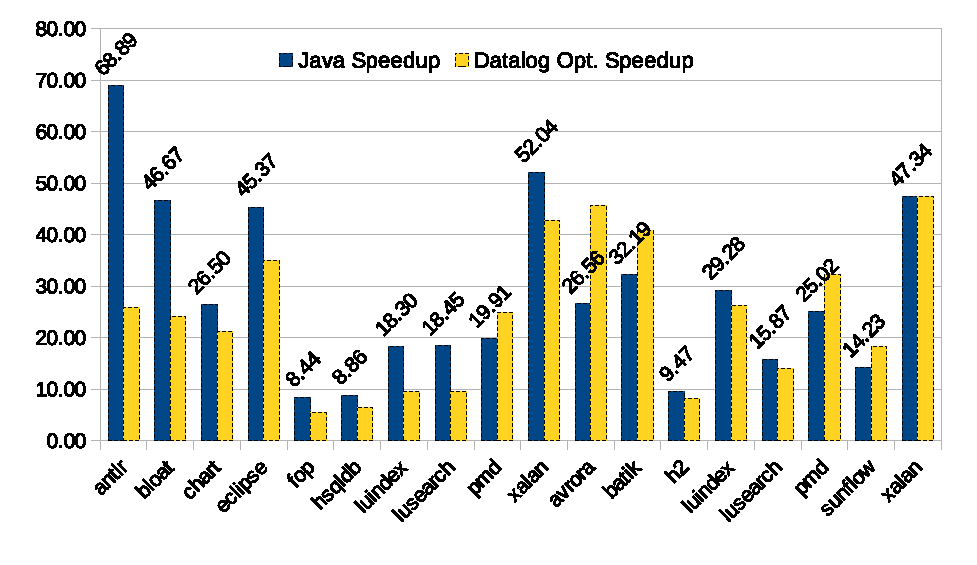
\includegraphics[clip,width=0.77\linewidth, height=0.4275\linewidth]{speedup.eps}
%%   \end{minipage}
%%   \caption{Speedup of the two analyses employing optimized data structure.}
%%     \label{fig:speedup}
%% \end{figure*}
%% 
%% 
%% 
%% It is not hard to see why the explicit representation is not competitive.
%% Figure~\ref{fig:pairs} correlates the number of aliased access-path pairs
%% (computed by the original analysis) and execution time.  (This applies to
%% context-qualified access paths, in the application and libraries alike, as long
%% as the library code is reachable from application code with the given context
%% depth.) This metric reflects the size (in tuples) of the corresponding relation
%% in the Datalog database. It clearly suggest that maintaining access path
%% relationships explicitly can prove quite costly.
%% 
%% \begin{figure}[h]
%%   \begin{minipage}[b]{\linewidth}
%%     \centering
%%     % left bottom right top
%%     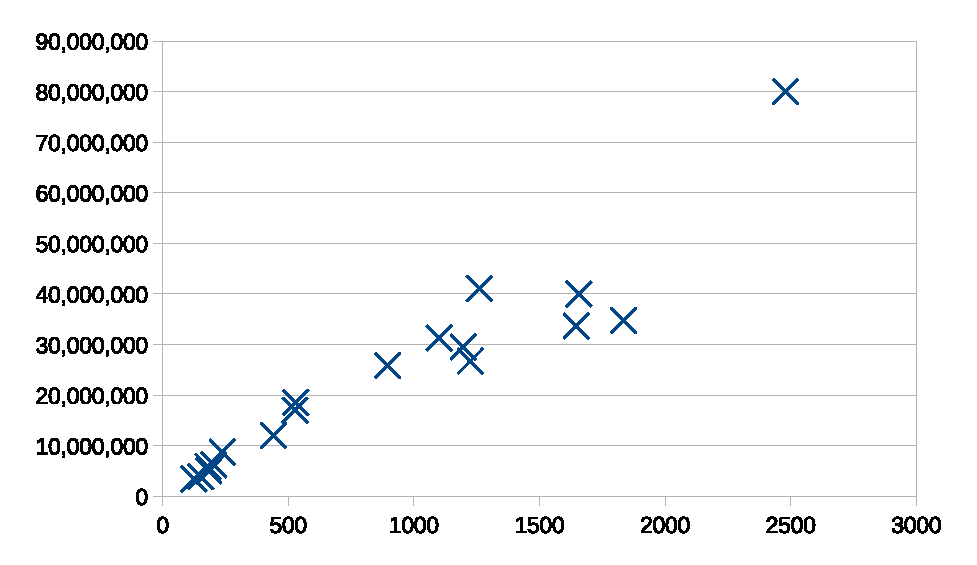
\includegraphics[clip,width=\linewidth]{pairs.eps}
%%   \end{minipage}
%%   \caption{Number of pairs of (instruction-and-context-qualified) access paths that must alias vs. analysis time.}
%%     \label{fig:pairs}
%% \end{figure}
%% 
%% %% Furthermore, the setup
%% %% explicitly downplays the benefits of our optimized data structure:
%% %% First, the ``optimized'' running time also includes import time and
%% %% computing must-point-to results for checking the equivalence of
%% %% analyses.  The latter is quite costly, since it requires re-expanding
%% %% the compactly-preserved access paths. The true computation times of
%% %% the optimized analysis are about one-third of the times listed in
%% %% Figure~\ref{fig:time}. Second, the configuration parameters (context
%% %% depth of 1 and access paths of at most length 2) are very modest, to
%% %% present the explicit representation in the best possible (while still
%% %% realistic) light. Changing these parameters can incur dramatic
%% %% slowdowns for the explicit representation, as we examine next.
%% 
%% 
%% \paragraph{Varying access-path length.} To further see the performance
%% advantage of the optimized representation of must-alias information, one can
%% vary the maximum access path length allowed for computations of the original,
%% explicit (Datalog) implementation.  Figure~\ref{fig:aplength} shows how running
%% time varies for maximum access path lengths of 2, 3 (same as in
%% Figure~\ref{fig:time}), 4 and 5. The numbers are for the xalan benchmark. The
%% speedup readily grows to over 75x for an allowed access path length of 5. The
%% optimized Datalog implementation is shown as a baseline although it should be
%% (and is) largely unaffected by the change of maximum access path length.
%% 
%% \begin{figure}[h]
%%   \begin{minipage}[b]{\linewidth}
%%     \centering
%%     % left bottom right top
%%     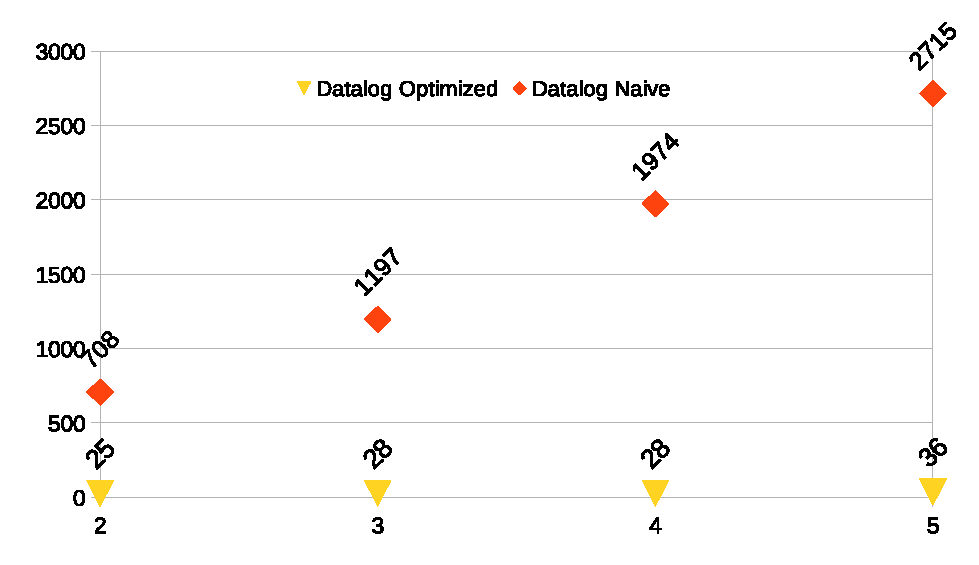
\includegraphics[clip,width=\linewidth]{length.eps}
%%   \end{minipage}
%%   \caption{Execution time when varying maximum access-path length. Optimized
%%     Datalog running time given as a baseline.}
%%     \label{fig:aplength}
%% \end{figure}
%% 
%% 
%% %for which the optimized representation achieved the \emph{lowest} speedup (14x) in Figure~\ref{fig:time}.
%% 
%% 
%% %% \begin{figure}
%% %%   \setlength{\tabcolsep}{6pt}
%% %%   \centering
%% %%   \begin{tabular}{||l| r| r| r| r| r||}
%% %%     \toprule
%% %%   Access path   &      optimized &      explicit & speedup  & must-alias & access path         \\
%% %%     length      & time  (sec)    & time (sec)    &          &  \#pairs   &  must-point-to   \\
%% %%                 &                &               &          &    (Ks)    &  \# entries  (Ks)\\
%% %%     \midrule
%% %%     1 &     47 & 290	                         & 6.2      & 	3399    & 	1953  \\
%% %%     2 &     47 & 658	                         & 14.0     & 	9979    &   1969  \\
%% %%     3 &     47 & 1521                            & 32.4     & 18528    & 	1971  \\
%% %%     \bottomrule
%% %%   \end{tabular}
%% %%   \caption{Analysis results (for the xalan benchmark) when varying the
%% %%     maximum access path length. This restriction does not affect our
%% %%     optimized implementation, whose running time is included in every
%% %%     row only for reference.}
%% 
%% %%   \label{fig:aplength}
%% %% \end{figure}
%% 
%% 
%% \paragraph{Varying context depth.} Similar observations can be made by varying
%% the context depth of the analysis. As seen in Figure~\ref{fig:ctxdepth},
%% although the running time of the optimized implementation grows slowly, the
%% running time of the explicit representation of alias relationships gets
%% dramatically higher. For a context depth of 4, the explicit representation did
%% not terminate after one-and-a-half hour.
%% 
%% \begin{figure}[h]
%%   \begin{minipage}[b]{\linewidth}
%%     \centering
%%     % left bottom right top
%%     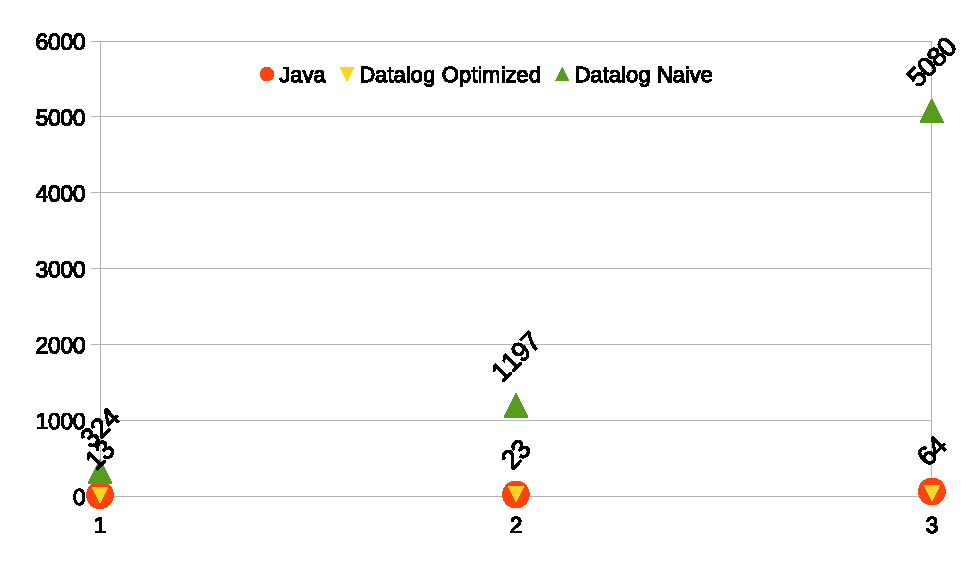
\includegraphics[clip,width=\linewidth]{depth.eps}
%%   \end{minipage}
%%   \caption{Execution time when varying maximum context depth.}
%%     \label{fig:ctxdepth}
%% \end{figure}
%% 
%% 
%% %% \begin{figure}
%% %%   \setlength{\tabcolsep}{6pt}
%% %%   \centering
%% %%   \begin{tabular}{||l| r| r| r| r| r||}
%% %%     \toprule
%% %%     Context   &      optimized &      explicit & speedup & must-alias & access path         \\
%% %%     depth     & time  (sec)    & time (sec)    &         &  \#pairs   &  must-point-to   \\
%% %%               &                &               &         &    (Ks)    &  \# entries (Ks) \\
%% %%     \midrule
%% %%     0 &  45 & 	92  & 	2.0	 &  1177 & 	1794 \\  
%% %%     1 &  47 & 	658 & 	14.0 & 	9979 & 	1969 \\  
%% %%     2 &  56 & 	1449&	25.9 &  33439&	2610 \\  
%% %%     \bottomrule
%% %%   \end{tabular}
%% %%   \caption{Analysis results (for the xalan benchmark) when varying the maximum
%% %%    context depth of the analysis.}
%% 
%% %%   \label{fig:context}
%% %% \end{figure}
%% 
%% Recall the two claimed benefits of the optimized representation: long access
%% paths are represented implicitly, and equivalence classes are represented with
%% linear space and time complexity, instead of quadratic. It is the latter factor
%% that comes into play when context depth increases: alias sets grow in size, by
%% exploiting inter-procedural inference (e.g., aliasing established at the caller
%% and propagated through formal arguments) in addition to local instructions.
%% 
%% In all, the optimized representation fulfills its promise of a much more
%% economical representation of must-alias (equivalence) relations. 
%% 
%% 
%% 
%% %% The minimal model of earlier sections captures the essence of our
%% %% full-fledged implementation. Our framework, \textsc{MaDoop}, is built
%% %% on top of the \textsc{Doop} Datalog framework for may-point-to
%% %% analysis of Java bytecode~\cite{oopsla:2009:Bravenboer}. Whereas
%% %% \textsc{Doop} is a flow-insensitive points-to analysis framework
%% %% (ignoring the order of instructions in a method), \textsc{MaDoop} adds
%% %% flow-sensitive modeling of the Java bytecode program (a full
%% %% control-flow graph over basic blocks). All program structure
%% %% information is represented as logical tables, which are subsequently
%% %% processed by about 300 logical rules.
%% 
%% 
%% %% To demonstrate the framework experimentally, we apply it to the DaCapo
%% %% benchmark programs~\cite{oopsla:2006:Blackburn} v.2006-10-MR2 under JDK
%% %% 1.7.0\_21.  We use the LogicBlox Datalog engine, v.3.10.19, on a Xeon
%% %% E5530 2.4GHz machine with only one thread running at a time and 24GB
%% %% of RAM.  When a may-analysis is needed, we employ the most precise
%% %% analysis that scales to large programs in the \textsc{Doop}
%% %% framework---a 2-object-sensitive analysis with a context-sensitive
%% %% heap (2objH).
%% 
%% %% We study five of the DaCapo benchmarks: antlr, chart, luindex,
%% %% lusearch, pmd. We wanted a small enough set for human inspection of
%% %% alias pairs at select program points, as well as programs for which a
%% %% 2objH analysis terminates. The scalability of our own must-alias
%% %% analysis is not a concern: as discussed earlier, a must-alias analysis
%% %% is naturally incremental. Hence, scalability to large programs is largely not
%% %% an issue: we can apply the analysis to just the application classes or
%% %% to a smaller hand-selected subset of the program code.
%% 
%% %% Figure~\ref{fig:info} presents statistics on the sizes of the
%% %% benchmarks, in terms of application code deemed reachable by the
%% %% \textsc{Doop} may-point-to analysis (2objH), as well as the running
%% %% time of this analysis. We also include the execution time for the
%% %% preparatory computation over the may-analysis results (``must
%% %% pre-analysis'' column)---i.e., the time to compute our
%% %% required input predicates, \altrelname{Resolved},
%% %% \altrelname{MayAlias} and \altrelname{CallMayStoreToField}.
%% 
%% %% %% \begin{figure}[t]
%% %% %%   \small
%% %% %%   \centering
%% %% %%   \begin{tabular}{lrrrrr}
%% %% %%     \toprule
%% %% %%     &&&& \multicolumn{2}{c}{may analysis time}
%% %% %%     \\
%% %% %%     \cmidrule(lr){5-6}
%% %% %%     Bench. & instructions & methods & classes & core (2objH) & must
%% %% %%                                                                   pre-analysis
%% %% %%     \\
%% %% %%     \midrule
%% %% %%     antlr    & 65518 & 1638 & 229 &  7m48s & 3m41s \\ %.18s \\
%% %% %%     chart    & 29126 & 1176 & 516 & 18m46s & 4m21s \\ %.07s \\
%% %% %%     luindex  & 19732 &  693 & 351 &   4m5s & 1m51s \\ %.90s \\
%% %% %%     lusearch & 26473 & 1049 & 351 &  4m28s & 1m58s  \\ %.78s \\
%% %% %%     pmd      & 49114 & 1880 & 554 &  5m25s & 3m18s \\ %.22s \\
%% %% %%     \bottomrule
%% %% %%   \end{tabular}
%% %% %%   \caption{Statistics for reachable application code, 2objH
%% %% %%     may-point-to analysis and must pre-analysis.}
%% %% %%   \label{fig:info}
%% %% %% \end{figure}
%% 
%% %% \begin{figure}[t]
%% %%   \small
%% %%   \centering
%% %%   \begin{tabular}{lrrrr}
%% %%     \toprule
%% %%     &&& \multicolumn{2}{c}{may analysis time}
%% %%     \\
%% %%     \cmidrule(lr){4-5}
%% %%     Benchmark & methods & classes & core (2objH) & must
%% %%                                                                   pre-analysis
%% %%     \\
%% %%     \midrule
%% %%     antlr    & 1638 & 229 &  7m48s & 3m41s \\ %.18s \\
%% %%     chart    & 1176 & 516 & 18m46s & 4m21s \\ %.07s \\
%% %%     luindex  &  693 & 351 &   4m5s & 1m51s \\ %.90s \\
%% %%     lusearch & 1049 & 351 &  4m28s & 1m58s  \\ %.78s \\
%% %%     pmd      & 1880 & 554 &  5m25s & 3m18s \\ %.22s \\
%% %%     \bottomrule
%% %%   \end{tabular}
%% %%   \caption{Statistics for reachable application code, 2objH
%% %%     may-point-to analysis and must pre-analysis.}
%% %%   \label{fig:info}
%% %% \end{figure}
%% 
%% %% Our must-alias analysis is run with a maximum access path length of
%% %% 3. Context depth varies per experiment, as discussed below.
%% 
%% %% \paragraph{Comparison with Intra-Procedural Analysis.}
%% 
%% %% As a first measure of the value of our inter-procedural must-alias
%% %% analysis, we compare it against intra-procedural analyses. Traditional
%% %% compilers can already compute aliases using intra-procedural data-flow
%% %% analysis and employ them for optimizations such as common
%% %% subexpression elimination, constant folding, or register allocation.
%% %% It is interesting to consider whether there is benefit from considering
%% %% more precisely the effects of called methods, in order to infer more
%% %% local aliases.
%% 
%% %% For this experiment, we ran our analysis algorithm (with a context
%% %% depth of 1) over the entire application portion of the
%% %% benchmarks. That is, the size of our \consname{RootMethod} set is the
%% %% number of methods shown in Figure~\ref{fig:info}.
%% 
%% %% The first and last settings shown in Figure~\ref{fig:exp1} (``intra-procedural'' and
%% %% ``inter-procedural'', respectively) present a
%% %% purely intra-procedural analysis and our full inter-procedural
%% %% algorithm.
%% %% %The former is
%% %% %produced from our framework with the inter-procedural propagation
%% %% %rules disabled. 
%% %% The intra-procedural analysis does not exploit aliasing
%% %% inferences from other methods, and conservatively invalidates alias
%% %% pairs at method calls and heap stores.
%% 
%% %% \begin{figure*}[t]
%% %%   \small
%% %%   \centering
%% %%   \begin{tabular}{lrcrrcrrcrrcr}
%% %%     \toprule
%% %%     \multicolumn{13}{c}{\normalsize \emph{Alias pairs}} \\
%% %%     % \cmidrule(l){2-13}
%% %%     \midrule
%% %%     & \multicolumn{3}{c}{intra-procedural}
%% %%     & \multicolumn{3}{c}{intra-proc.$^{+\text{may}}$}
%% %%     & \multicolumn{3}{c}{inter-proc.$_{-\text{may}}$}
%% %%     & \multicolumn{3}{c}{inter-procedural} \\
%% %%     \cmidrule(lr){2-4} \cmidrule(lr){5-7} \cmidrule(lr){8-10} \cmidrule(l){11-13}
%% %%     & \multirow{2}{2em}{per insn.} & \multirow{2}{2em}{per ret.} & time
%% %%     & \multirow{2}{2em}{per insn.} & \multirow{2}{2em}{per ret.} & time
%% %%     & \multirow{2}{2em}{per insn.} & \multirow{2}{2em}{per ret.} & time
%% %%     & \multirow{2}{2em}{per insn.} & \multirow{2}{2em}{per ret.} & time
%% %%     \\ Bench. \\
%% %%     \midrule
%% %%     antlr    &  7 &  3 & 1m37s & 41 &  6 & 3m21s &  34 & 19 & 14m25s & 105 & 27 & 37m37s \\
%% %%     chart    & 10 &  4 & 1m37s & 15 &  6 & 1m34s &  26 & 20 &  3m31s & 34 & 24  &  4m57s \\
%% %%     luindex  &  4 &  3 & 0m36s &  7 &  6 & 0m59s &   7 &  7 &  1m26s & 12 & 12  &  1m34s \\
%% %%     lusearch &  5 &  3 & 0m53s &  6 &  5 & 0m54s &   8 &  6 &  1m22s & 12 & 10  &  1m56s \\
%% %%     pmd      & 13 &  3 & 2m26s & 15 &  4 & 2m19s &  23 & 17 &  7m59s & 27 & 19  &  9m39s \\
%% %%     \bottomrule
%% %%   \end{tabular}
%% %%   \caption{Average \#alias pairs per program element (divided by 2,
%% %%     i.e., with equivalent symmetric pairs removed), and timings for
%% %%     various settings.}
%% %%   \label{fig:exp1}
%% %% \end{figure*}
%% 
%% %% The main metric to watch for in this comparison is ``alias
%% %% pairs per instruction'', i.e., the first of the three columns in every
%% %% grouping of numbers. As can be seen, the full inter-procedural analysis
%% %% (last of the four settings shown in Figure~\ref{fig:exp1}) yields
%% %% significantly richer information than the intra-procedural analysis
%% %% (first setting). With only intra-procedural information, we can infer
%% %% at most one half, and often less than one third, of the alias pairs.
%% %% The alias pairs shown are unconditional (i.e., for context
%% %% \consname{All}) with symmetric pairs removed. The numbers are over the
%% %% Jimple intermediate language of the Soot framework and, thus, the
%% %% alias pairs are more numerous than one would expect from program
%% %% inspection, due to the introduction of several temporary
%% %% variables. 
%% 
%% %% \begin{figure*}[t]
%% %%   \small
%% %%   \centering
%% %%   \begin{tabular}{lrrrrrr}
%% %%     \toprule
%% %%     & \multicolumn{3}{c}{\emph{Alias pairs} under 1-must-context}
%% %%     & \multicolumn{3}{c}{\emph{Alias pairs} under 5-must-context} \\
%% %%     \cmidrule(lr){2-4} \cmidrule(lr){5-7}
%% %%     Benchmark & per instr. & per all-return & time
%% %%               & per instr. & per all-return & time
%% %%     \\
%% %%     \midrule
%% %%     antlr    & 10 &  8 & 0m51s & 19 & 12 &  2m48s \\
%% %%     chart    & 25 & 13 & 1m25s & 30 & 18 &  1m21s \\
%% %%     luindex  &  8 &  6 & 0m20s &  9 &  7 &  0m25s \\
%% %%     lusearch &  6 &  5 & 0m22s &  9 &  7 &  1m12s \\
%% %%     pmd      &  6 &  4 & 0m25s & 11 &  9 & 10m12s \\
%% %%     \bottomrule
%% %%   \end{tabular}
%% %%   \caption{Alias pairs (with equivalent symmetric pairs removed, i.e., numbers divided by 2), and timings
%% %%   for different contexts of the must-alias analysis.}
%% %%   \label{fig:exp2}
%% %% \end{figure*}
%% 
%% 
%% %% \paragraph{Value of May-Analysis for Must- Inference.}
%% 
%% %% Figure~\ref{fig:exp1} shows two more settings of our analysis:
%% %% intra-procedural$^{+\text{may}}$ and inter-procedural$_{-\text{may}}$.
%% %% These help us quantify how exactly may-analysis information
%% %% contributes to the must-analysis.
%% 
%% %% The intra-procedural$^{+\text{may}}$ setting does intra-procedural
%% %% must-alias reasoning but invalidates access paths by employing the
%% %% inter-procedural may-alias analysis. That is, of the three predicates
%% %% computed by the may-analysis, the intra-procedural$^{+\text{may}}$
%% %% analysis does \emph{not} use predicate \altrelname{Resolved} to do
%% %% virtual method resolution, but \emph{does} use predicates
%% %% \altrelname{MayAlias} and \altrelname{CallMayStoreToField}, in order
%% %% to decide when to invalidate access paths at call and store
%% %% instructions. 
%% %% %
%% %% Conversely, the inter-procedural$_{-\text{may}}$ analysis \emph{does}
%% %% use predicate \altrelname{Resolved} to do virtual method resolution,
%% %% but does \emph{not} use predicates \altrelname{MayAlias} and
%% %% \altrelname{CallMayStoreToField}, instead invalidating alias
%% %% information conservatively at store and call instructions.
%% 
%% %% These variations of settings give us a picture of the separate benefit
%% %% from various kinds of inter-procedurality (may vs. must reasoning).
%% %% As can be seen, inter-procedural reasoning benefits greatly from both
%% %% kinds of inter-procedural may-analysis information. 
%% %% %%SPACE
%% %% %The inter-procedural$_{-\text{may}}$ setting is significantly less
%% %% %effective than the full inter-procedural analysis, while still
%% %% %typically much better than intra-procedural$^{+\text{may}}$, which, in
%% %% %turn, is better than the purely intra-procedural setting.
%% %% %
%% %% %%SPACE
%% %% Note that all of the above configurations were produced via
%% %% straightforward configuration of our full implementation.
%% %% This is testament to the inherent configurability of a modular,
%% %% declarative framework.
%% %% %This ease of
%% %% %experimentation is testament to the inherent configurability of a
%% %% %modular, declarative framework, as opposed to a monolithic
%% %% %implementation.
%% 
%% %% \paragraph{Timings.}
%% 
%% %% Figure~\ref{fig:exp1} also shows the running time for our analysis, as
%% %% well as for intra-procedural analyses. As can be seen, the must-alias
%% %% analysis is quite fast. In the case of antlr, the analysis time blows up,
%% %% but so do the inferred facts. Generally, our timings do not aim
%% %% to reflect an ideal implementation of the declarative
%% %% rules. Specifically, our Datalog
%% %% engine does not use union-find trees for the equivalence classes of
%% %% reflexively and transitively closed relations, thus incurring
%% %% significant overhead.
%% %% %We have tried to minimize such overhead within the parameters allowed
%% %% %by the execution engine but a manual implementation can likely fare
%% %% %better. 
%% %% On the other hand, our implementation is heavily optimized in terms of
%% %% rule execution and indexing (for fast combination of relations), to an
%% %% extent that a manual implementation will have difficulties matching.
%% 
%% 
%% %% \paragraph{Results for Human Inspection.}
%% 
%% %% For human inspection of aliases, we have found it useful to produce
%% %% all alias pairs that hold (unconditionally, i.e., under an
%% %% \consname{All} context) for \emph{all} return statements of a method.
%% %% This ``forall'' intersection of aliasing information over all
%% %% return sites offers a good summary of the method's effects, and
%% %% is more concise than alias information at a single given
%% %% instruction.
%% 
%% %% Figure~\ref{fig:exp1} shows the sizes of the sets computed in this
%% %% fashion, as the second of the three columns for every analysis
%% %% setting.  As can be seen, the full inter-procedural must-alias
%% %% analysis is again significantly more information-rich than any other
%% %% setting. The sizes of the resulting alias sets (from 10 to 27)
%% %% are small enough for human inspection and typically
%% %% quite informative.
%% 
%% 
%% 
%% %% \paragraph{Exploring Parts of the Program, Using Context.}
%% 
%% %% To explore parts of the program only conditionally (with alias pairs
%% %% qualified by context), we selected at random 20 methods in each of the
%% %% benchmarks. We ran the analysis with these methods in the
%% %% \consname{RootMethod} set, and different maximum context depth values,
%% %% to allow exploration of code outside that set as much as the context
%% %% depth permits.
%% 
%% %% Figure~\ref{fig:exp2} shows the result of this experiment, for context
%% %% depth settings of 1 and 5. The alias pairs shown are computed \emph{at
%% %%   the root methods only}, i.e., they do not count alias pairs in the
%% %% methods analyzed under a non-\consname{All} context, but they do count
%% %% the impact of such methods on the alias information at the original
%% %% root method set.
%% 
%% %% The execution time demonstrates the incrementality of the must-alias
%% %% analysis---its running time was often negligible.
%% %% %%SPACE
%% %% % (Recall that much of
%% %% %the time shown is spent computing queries over the \emph{may-}
%% %% %analysis, in order to populate input tables \altrelname{Resolved},
%% %% %\altrelname{MayAlias}, and \altrelname{CallMayStoreToField}, and not
%% %% %on the must-alias analysis itself.)
%% 
%% %% For a deeper context, the analysis produces often significantly richer
%% %% facts. Since the methods of origin are randomly selected, the number of
%% %% extra alias pairs (when mapped back at the root
%% %% methods) varies, but is generally consistent.






%% \section{Conclusions}
%% \label{sec:conclusions}

%% We presented a declarative algorithm model for an inter-procedural
%% must-alias analysis over access paths, and a data structure for its
%% optimized implementation. The algorithmic improvements afforded
%% by the specialized data structure yield a tremendous performance
%% advantage, often approaching two orders of magnitude.

%% The literature on must-alias analyses is sparse and the distance of
%% specification to implementation is typically large. In our literature
%% survey we have not found a single must-alias analysis publication that
%% concretely refers to another and shows how its approach differs. Thus,
%% we believe that our declarative model can offer a reference point for
%% future work. Accompanied by our proposed data structure, the model can
%% spur further discussion on how to make must-alias analyses more
%% complete and how to implement them efficiently.

%\newpage

%% We believe that our model is clear yet concrete
%% enough to spur further development and a better understanding of the
%% comparative features of different must-alias analysis algorithms. In
%% practical terms, must-alias analysis is valuable and woefully
%% under-exploited in the literature. Our experiments show concrete value
%% for (human) program understanding and (automatic) optimization.


%% discussed its features and configurability options.  The
%% model faithfully reflects \textsc{MaDoop}: a full-fledged
%% implementation of more than 300 Datalog rules to analyze Java
%% bytecode. Our analysis interfaces with the may-point-to analyses of
%% the \textsc{Doop} framework and can leverage their precision, at
%% clearly defined interaction points.
